\documentclass[11pt]{article}

\usepackage[margin=0.9in]{geometry}
\usepackage{graphicx}
\usepackage{gensymb}
\usepackage{multicol}
\usepackage{amsfonts,amsmath,amssymb}
\usepackage{epstopdf}
\usepackage{tabularx,colortbl}
\usepackage[none]{hyphenat}
\usepackage{fancyhdr}
\usepackage{float}
\usepackage{hhline}
\usepackage{graphicx}
\usepackage{eurosans}
\usepackage{caption}
\usepackage{float}
\usepackage{fourier} 
\usepackage{array}
\usepackage{makecell}
\usepackage[nottoc,notlot,notlof]{tocbibind}
\usepackage{graphicx}
\usepackage{colortbl,booktabs}
\usepackage{xcolor}
\newenvironment{rcases}
  {\left.\begin{aligned}}
  {\end{aligned}\right\rbrace}
\usepackage[]{hyperref}
%\renewcommand\theadalign{bc}
%\usepackage{float}
\newcolumntype{P}[1]{>{\centering\arraybackslash}p{#1}}
\newcolumntype{M}[1]{>{\centering\arraybackslash}m{#1}}
\DeclareCaptionType{mycapequ}[][List of equations]
\captionsetup[mycapequ]{labelformat=empty}
\definecolor{gray}{rgb}{0.85,0.85,0.85}
\pagestyle {fancy}

\fancyhead {}

\fancyfoot {}

\fancyhead [L] {\slshape \MakeUppercase{ 6U Cubesat}}

%\fancyhead [R] {\slshape Innocente Andrea Contalbo}

\fancyfoot [C] {\thepage}

\renewcommand{\footrulewidth}{0pt}



\parindent 0ex

\renewcommand{\baselinestretch}{1}






\rhead{\vspace{-0.5cm}
\includegraphics[width=0.3\textwidth]{newlogo.eps}}


\begin{document}
\lfoot{AY 2018-19 -- Prof.\ J.\ D.\ Biggs}



\begin{titlepage}

\begin{figure} [H]

\centering 


\includegraphics[scale=0.5]{poli.png}

\end{figure}

\begin{center}

\vspace{1cm}

\Large{\textbf{Department of Aerospace Science and Technology}}\\

%\Large{\textbf{Class Laboratory 1}}\\

\vfill

\line(1,0){400}\\[1mm]

\huge{\textbf{ 6U Cubesat\\Detumbling, Slew Manoeuvre and Sun Pointing}}\\ [3mm]

\Large{\textbf{ Spacecraft Attitude Dynamics And Control \\ Final Project}}\\ [1mm]

\line(1,0) {400}\\

\begin{figure} [H]

\centering 

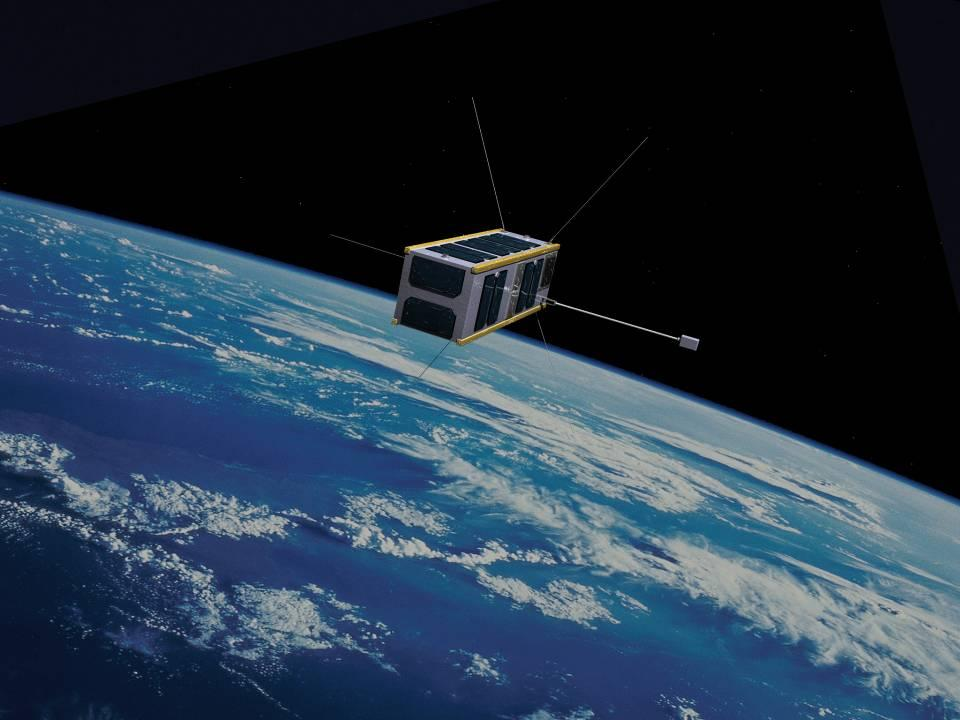
\includegraphics[scale=0.4]{cubesat-1.jpg}

\end{figure}

\vfill

%Andrea De Vittori 898352\\

%Candidate \#899783\\

%\today\\

\end{center}

\end{titlepage}



\tableofcontents

\thispagestyle {empty}

\clearpage

%\twocolumn

\setcounter{page}{1}



\section{Introduction}

A CubeSat (U-class spacecraft) is a  miniaturized satellite  made for space purposes and is composed by  multiples of $10\times10\times10$ cm cubic units. The mass is no more than 1.33 kilograms per unit,and often characterized by commercial off-the-shelf (COTS) components for their electronics and structure. CubeSats are commonly put in orbit by deployers on the International Space Station, or launched as secondary payloads on a launch vehicle. The intent is to  provide  affordable  access  to  space  for  the  university  science  community, Government agencies and commercial groups thanks to a standardized design of the whole structure. Uses typically involve experiments that can be miniaturized or serve purposes such as Earth observation \cite{intro}. Concerning the 6U (adopted in this project) is essentially the same as two 3Us side-by-side, making it twice as wide . Here listed there are the main features of the mission ,  deepened and developed through the project:
\begin{enumerate}
\item The satellite is set on a GEO orbit whose aim, after the de-tumbling phase, is to point the Sun.
\item The de-tumbling relies on a magnetometer and on a gyro for the attitude and dynamics determination.\\ Subsequently for slew and pointing only the magnetometer is allowed to perform the reconstruction of the the attitude matrix.
 \item Since ,After several attempts with 1 magneto torquers, the Cubesat is not able to de-tumble in a reasonable time span,as an exception, 4 Cold-Gas thrusters are located at the base of the spacecraft itself.
Regarding the control actuation ,for the last part of the mission, the system is fitted  with 4 reaction wheels.

\clearpage
\section{List of Parameters}

\subsection{Legend:}
This is the convention adopted for representing scalar, vector and matrix quantities:
\begin{multicols}{3}
\begin{enumerate}
    \item $a$ = scalar representation
    \item $\mathbf{a}$ = vector representation
   \item $\mathbf{A}$ = matrix representation
\end{enumerate}
\end{multicols}
\end{enumerate}
\subsection{List of selected data for the Simulink simulation:}

\begin{table}[H]
\centering
 \begin{tabular}{|M{2cm}|M{5cm}|M{6cm}|M{2cm}|}\hline
 \rowcolor{gray} 
  \textbf{Variable} & \textbf{Description} & \textbf{Value} & \textbf{Unit of measure}\\

\hhline{|=|=|=|=|}
$a_{geo}$ &initial semi major axis & 42164 & $[km]$\\
\hline
$e_{geo}$ & initial eccentricity & 0 & $[-]$\\
\hline
$i_{geo}$ &initial inclination & 0 & $[rad]$\\
\hline
$\omega_{geo}$ & initial anomaly of perigee & 0 & $[rad]$\\
\hline
$\Omega_{geo}$ &initial right ascension of the ascending node & 0 & $[rad]$\\
\hline
$\theta_{geo}$ & initial true anomaly & 0 & $[rad]$\\
\hline
$\boldsymbol{\omega_1}$ & initial angular velocity vector for detumbling & $\begin{bmatrix}
0.22 & 0.26 & 0.22
\end{bmatrix}$& $[rad/s]$\\
\hline
$\boldsymbol{\omega_2}$ & initial angular velocity vector for Slew & $10^{-4}\begin{bmatrix}
4.31   & 3.31  & -3.08
\end{bmatrix}$& $[rad/s]$\\
\hline
$\boldsymbol{\omega_3}$ & initial angular velocity vector for Pointing & $10^{-5}\begin{bmatrix}
  -0.36 &   0.34 &  -0.66
\end{bmatrix}$& $[rad/s]$\\
\hline
$\mathbf{A_1}$ & initial attitude matrix for de-tumbling & $\begin{bmatrix}
0.5335 & 0.808 &0.25 \\
    -0.808 & 0.3995 & 0.433\\
    0.25 & -0.433 & 0.866
\end{bmatrix}$& $[-]$ \\
\hline
$\mathbf{A_2}$ & initial attitude matrix for Slew & $\begin{bmatrix}
    0.4777  & -0.0636  &  0.8762\\
   -0.7262  &  0.5327   & 0.4345\\
   -0.4944  & -0.8439   & 0.2083
\end{bmatrix}$& $[-]$ \\
\hline
$\mathbf{A_3}$ & initial attitude matrix for Pointing & $\begin{bmatrix}
     0.8660 &   0.4589  &  0.1989\\
   -0.4996  &  0.7757 &   0.3856\\
    0.0226  & -0.4333   & 0.9009
\end{bmatrix}$& $[-]$ \\
\hline
$T_{detumbling}$ & integration time of detumbling & 180 & $[s] $\\
\hline
$T_{slew}$ & integration time of slew & 140 & $[s] $\\
\hline
$T_{pointing}$  & integration time of pointing & 86400 & $[s] $\\
\hline
M & mass of the Cubesat & 12 & $[Kg] $\\
\hline
w & width of the Cubesat & 226.3 & $[mm]$\\
\hline
l & length of the Cubesat & 100 & $[mm]$\\
\hline
a & heigth of the Cubesat & 366 & $[mm]$\\
\hline
$\mathbf{I}$ & Inertia matrix & $\begin{bmatrix}
0.218&0&0\\
0&0.166&0\\
0&0&0.082
\end{bmatrix}$& $[Kgm^2]$ \\
\hline
$f_g$ &  Gyro frequency & 262 & $[Hz]$\\
\hline





\end{tabular}
\end{table}

\begin{table}[H]
\centering
 \begin{tabular}{|M{2cm}|M{5cm}|M{6cm}|M{2cm}|}
\hline
 \rowcolor{gray} 
  \textbf{Variable} & \textbf{Description} & \textbf{Value} & \textbf{Unit of measure}\\

\hhline{|=|=|=|=|}
$\sigma_n$ & Gyro Noise  & 0.15 & $[\degree/ \sqrt{h}]$\\
\hline
$\sigma_b$ & Gyro Bias  & 0.3 & $[\degree/ h]$\\
\hline
$\sigma_w^2$ & diagonal term of $\mathbf{R}$  & $10^{-8}$ & $[rad^2/s^4]$\\
\hline
$\sigma_v^2$ & diagonal term of $\mathbf{Q}$  & $10^{-8}$ & $[rad^2/s^2]$\\
\hline
$f_m$ &  Magnetometer frequency & 18 & $[Hz]$\\
\hline
$p_{acc}$ & Magnetometer pointing acc.  & 30 & $[arcmin]$\\
\hline
$m_{mt}$ & Magnetic moment of the magneto torquer & 1.2 & $[Am^2]$ \\
\hline
$\mathbf{m_{SC}}$ & parasitic magnetic moment  & $\begin{bmatrix}
0.1 & 0.1 & 0.1 
\end{bmatrix}$ & $[Am^2]$\\
\hline
$m_{max}$ & maximum  torque of a RW & 1 & $[mNm]$\\
\hline
$\mathbf{A}$& matrix disposition of the reaction wheels &$\begin{bmatrix}
1&0&0&\frac{1}{\sqrt[]{3}}\\
0&1&0&\frac{1}{\sqrt[]{3}}\\
0&0&1&\frac{1}{\sqrt[]{3}}
\end{bmatrix}$& [-]\\
\hline
$\mathbf{A^*}$ & pseudo inverse of $\mathbf{A}$ & $\begin{bmatrix}
\frac{5}{6}&-\frac{1}{6}&-\frac{1}{6}\\
-\frac{1}{6}&\frac{5}{6}&-\frac{1}{6}\\
-\frac{1}{6}&-\frac{1}{6}&\frac{5}{6}\\
\frac{1}{2\sqrt[]{3}}&\frac{1}{2\sqrt[]{3}}&\frac{1}{2\sqrt[]{3}}
\end{bmatrix}$& [-]\\
\hline
$RL_{RW}$ & rate limiter of a RW & 10 & $[mNm/s]$\\
\hline
$m_{max}$ & max transmitted torque & 1 & $[mNm]$\\
\hline
$M_{st}$& max momentum storage for RW & 10 & $[mNms]$\\
\hline
F & Thrust of a Cold-Gas thruster & 10 & $[mN]$\\
\hline
$\tau_{Cold-Gas_{rise}}$&rise time for the Cold-Gas thruster & 10 & $[ms]$\\
\hline
$\tau_{Cold-Gas_{fall}}$&fall time for the Cold-Gas thruster & 50 & $[ms]$ \\
\hline
$\tau_{Cold-Gas_{delay}}$&delay time for the Cold-Gas thruster & 5 & $[ms]$\\
\hline
\
$\epsilon_{Cold-Gas}$&minimum value of $\omega$ to avoid chattering & $5 \cdot 10^{-4}$& $[rad/s]$\\
\hline
$\mathbf{C}$ & sensor matrix of the Kalman filter & $$\begin{bmatrix}
1&0&0\\
0&1&0\\
0&0&1
\end{bmatrix}$$& $[-]$\\
\hline
$k_{DCM}$& tuning parameter for the DCM filter & 0.1& [-]\\
\hline
$k_1$& prop.coeff of $\omega_e$ for the ideal control & 0.15 & $[Nm/rad]$\\
\hline
$k_2$& prop.coeff related to $\mathbf{A_e}$ for the ideal control & 0.005 & $[Nm]$\\
\hline
$r_{sun}$& distance Earth-Sun & 149600000 & $[km]$\\
\hline
B& Initial phase of the Sun & $\frac{\pi}{6}$ & $[rad]$\\
\hline
\end{tabular}
\end{table}







\clearpage


\section{Structure}
The physical dimensions of the spacecraft are  depicted by the following image \ref{dimension}: 
\begin{figure} [H]
\begin{minipage}[b]{.68 \textwidth}


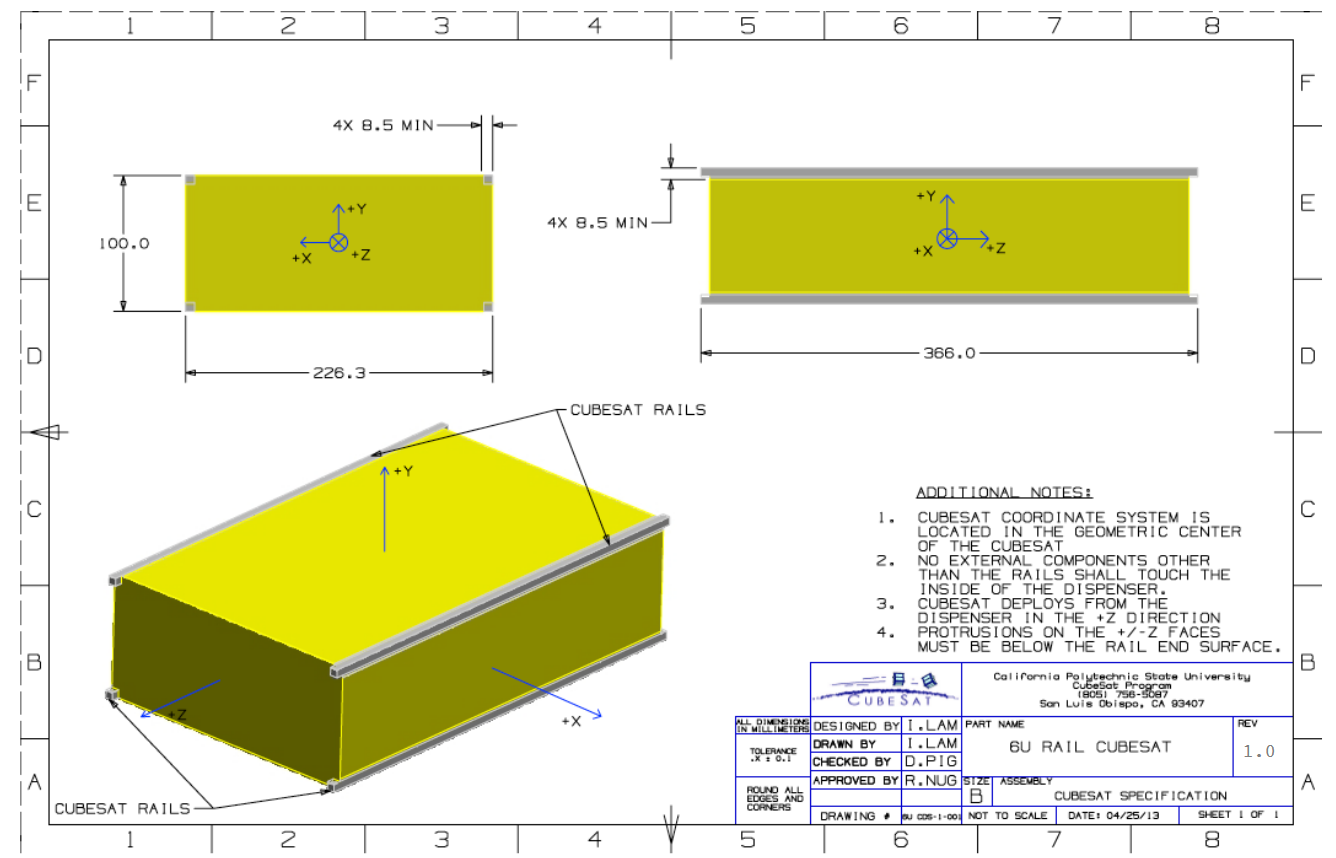
\includegraphics[width=\textwidth]{Geometry.PNG}


\caption{ 6U Cubesat dimensions specification \cite{6u dimension}}
\label{dimension}

\end{minipage}
\begin{minipage}[b]{.37 \textwidth}

\centering 

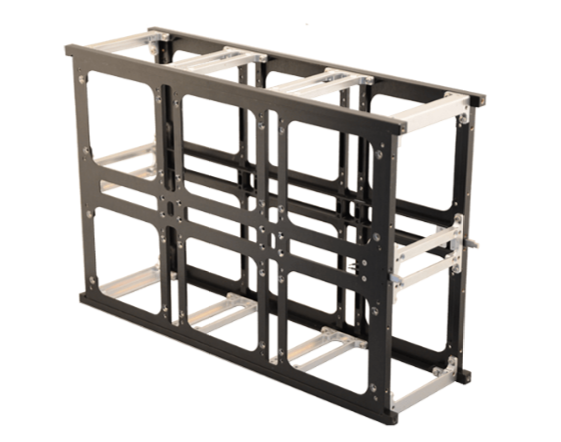
\includegraphics[width=\textwidth]{box.PNG} 
\caption{ 6-Unit cubesat structure
\cite{structure}}
\label{structures}
\end{minipage}
\end{figure}

The ISIS 6-Unit CubeSat \ref{structures} structure is developed as a modular satellite structure based upon the CubeSat standard. The design created by ISIS allows for multiple  configurations, giving CubeSat developers maximum flexibility in their design process.The hardware can be mounted directly inside with stacks or on the frame itself. Every device on board is accessible before mounting external hardware surfaces. Here the main features are shown  \cite{structure}:
\begin{multicols}{2}
\begin{itemize}
\item cost: \euro{7350}
\item Outside Envelope $ (l\times w\times h) \ 100\times 226.3 \times 366 \ mm $
\item Primary + Secondary Structure Mass 	1.1 kg
\item Inside Envelope $(l\times w\times h) \ per \ module (6 \times) \	96\times 96 \times 89.4 	\ mm$
\item Thermal Range (min $-$ max) -40 to +80 	\degree C
\end{itemize}
\end{multicols}



\section{ADCS architecture :}
\subsection{On board instrumentation:}
\subsubsection{gyro:}
\begin{minipage}{.4\textwidth}
\begin{figure} [H]

\centering 

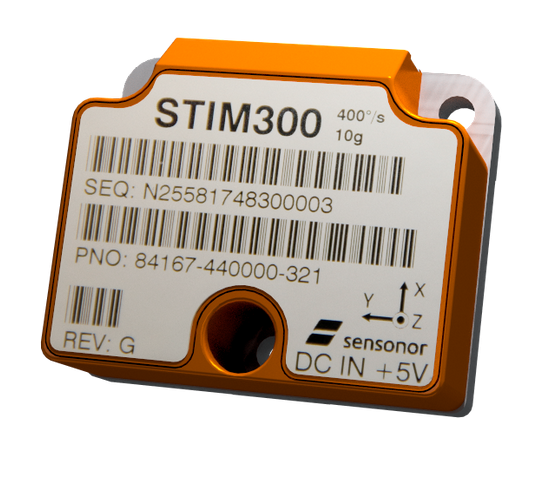
\includegraphics[scale=0.34]{Gyro.PNG}
\caption{ STIM300
\cite{gyro}}
\label{gyro}
\end{figure}
\end{minipage}
\begin{minipage}{.6 \textwidth}
The gyro works during the de-tumbling part for the dynamic determination.It measures the angular velocity of the satellite.STIM300 is a small, tactical grade, low weight, high performance non-GPS aided Inertial Measurement Unit (IMU). It contains 3 highly accurate MEMS gyros, 3 high stability accelerometers and 3 inclinometers. The IMU is factory calibrated and compensated over its entire operating temperature range.
\end{minipage}

  \begin{multicols}{2}
\begin{itemize}
\item cost: \euro{\ n.d}
\item   Update rate:  262Hz
\item   Bias: $<$ 0.3\degree/ h\
\item  Noise: $ <$ 0.15\degree/$\sqrt[]{h}$
\item  Volume: $35 \ cm^3$
\item  Mass:  0.55kg
\item    nominal Power:1.5 W
\item    Thermal (operational): -40 \degree C to +85 \degree C
\item Insensitive to magnetic fields   


\end{itemize}
\end{multicols}
\subsubsection{magnetometer:}
\begin{minipage}{.5 \textwidth}
 \begin{figure} [H]

  \centering 

  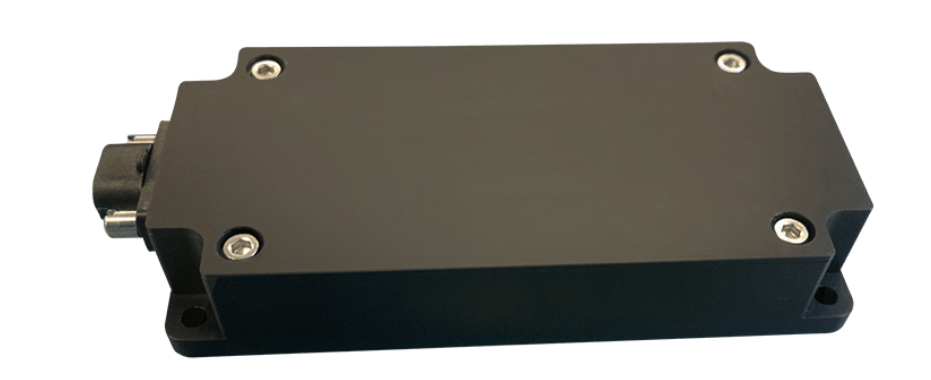
\includegraphics[scale=0.4]{magnetometer.PNG}



  \caption{ NSS Magnetometer
  \cite{magnetometer}}
  \label{magnetometer}
  \end{figure}
\end{minipage}
 \begin{minipage}{.5 \textwidth}
 The sensor provides x, y and z-axes magnetic field component measurements, in the body reference frame.Mounted outside the spacecraft at the end of a rigid boom the NewSpace Systems magnetometer includes low noise, precision processing and analogue-to-digital conversion circuitry. By knowing the local magnetic field of the Earth it is capable of measuring the attitude kinematics of the spacecraft.Furthermore it is useful  for the calculation of magnetorquer rods control torque levels. 

 \end{minipage}\\\\

\begin{multicols}{2}
\begin{itemize}
\item cost: \euro{14790}
\item    Measurement range: -60,000 nT to +60,000 nT
\item   Update rate: $<$ 18Hz
\item   Resolution: $<$ 8 nT
\item Pointing accuracy: 0.5 \degree
\item  Dimensions: $96\times 43 \times 17mm$
\item  Mass: $<$ 85g
\item    Power:$ < $ 750mW
\item    Thermal (operational): -25\degree C to +70 \degree C
\item Power supply: +5V DC
    


\end{itemize}
\end{multicols}


\subsection{Actuators:}
\subsubsection{Magneto torquer:}
\begin{figure} [H]

\centering 

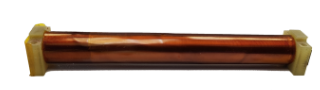
\includegraphics[scale=0.8]{Magneto_torquers.PNG}


\caption{ NCTR-M012 Magnetorquer Rod
\cite{magneto_torque}}
\label{rod}
\end{figure}

Magnetorquers offer a way of controlling the attitude of a satellite. This can be attained  by means of the interaction of  the local Earth's magnetic field.

Operating a magnetic alloy rod produces an amplification effect over an air cored magnetorquer. This requires less power, which is critical for CubeSat missions. The rods can enable a mission with increased manoeuvrability and reduced detumble rates.

CubeSat Magnetorquer rods are designed to be run directly from a switched 5 Volt power output from the on-board power control system.\\In the assigned project only 1 Magnetotorquer is provided with these properties \cite{magneto_torque}:
\begin{multicols}{2}
\begin{itemize}
\item cost: \euro{1750}
\item Magnetic moment: $1.2 Am^2$
\item Residual moment: $<$ $0.002 Am^2$
\item Operating range: -10 \degree C to +50 \degree C
\item Power: 5 Volt
\item Lifetime: $>$ 10 years
\item Dimensions: 94mm x 15 mm x 13 mm
\item Mass: $<$ 50 g

\end{itemize}
\end{multicols}

This particular rod \ref{rod} has some benefits to take into account . First things first it is a 
low cost standard product, it guarantees
high moment for low power and  is featured by
small size and low mass , crucial for nano-satellites. In addition it has no residual moment.



\subsubsection{Reaction wheels:}
\begin{figure} [H]

\centering 

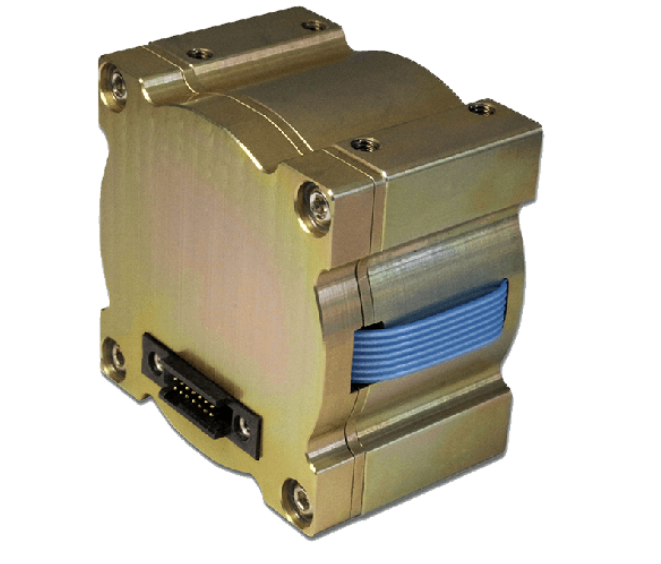
\includegraphics[scale=0.38]{RW.PNG}


\caption{ CubeWheel Medium
\cite{reaction_w_medium}}
\label{RW_medium}
\end{figure}
The CubeWheel Medium is a reaction wheel adopted to control the attitude of nanosatellites. The  module contains a brushless DC motor with vacuum-rated bearings, as well as the required drive electronics and speed control algorithms. Specs:
\begin{multicols}{2}
\begin{itemize}
\item cost: \euro{5,400}
\item Max torque: 1.0 mNm
\item  Average power consumption: $<$180 mW (@2000 RPM, 8V)
\item momentum storage : 10 mNms
\item  Mass: 130 g
\item  Operating voltage: 3.3V / battery voltage (6.5V to 16V) \item Dimensions: 46 x 46 x 31.5 mm
 \item mountable in 3 axis


\end{itemize}
\end{multicols}
\begin{minipage}{.5\textwidth}
\begin{figure} [H]

\centering 

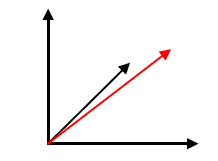
\includegraphics[scale=0.8]{pyramid.PNG}


\caption{ Reaction wheels layout
\cite{reaction_w}}
\label{RW}
\end{figure}
\end{minipage}
\begin{minipage}{.5\textwidth}
To work properly , during the slew and pointing phase of the mission , the reaction wheels should be at least 3 mounted on the axes. In case of redundancy a fourth momentum wheel could be added with the following layout \ref{RW}. Whenever one of the 3 rotors fails the fourth still guarantees controllability.
\end{minipage}

\subsubsection{Cold-Gas Thrusters}
\begin{figure} [H]

\centering 

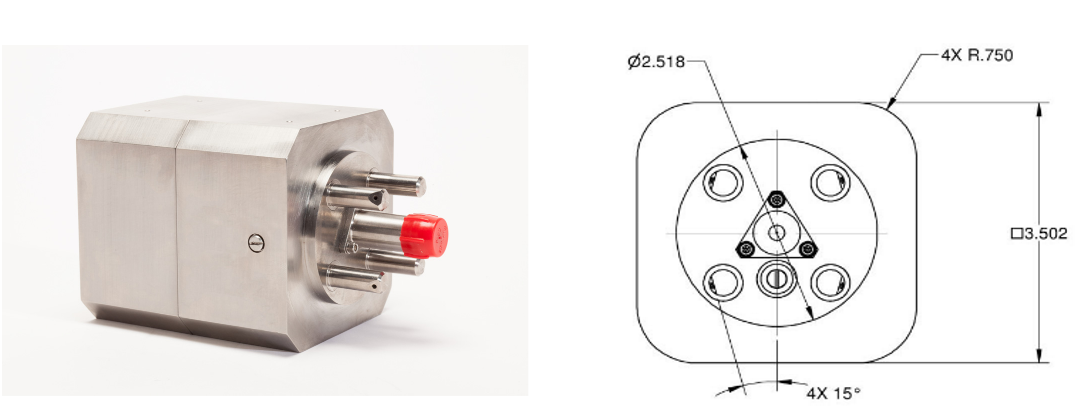
\includegraphics[scale=0.6]{Vacco.PNG}


\caption{ CubeWheel Medium
\cite{Vacco}}
\label{Vacco}
\end{figure}



The  VACCO   CubeSat  Hybrid  ADN
 Reaction  Control  System  is  a  high
performance  micro  propulsion  system  (MiPS)
specifically designed for CubeSats. The smart feed system automatically provides closed-loop thrust vector control during delta-v burns. Reliability is ensured through simplicity of design, welded titanium construction and frictionless valve technology.
\begin{multicols}{2}
\begin{itemize}
\item cost: nd
\item Smart, self-contained propulsion system
\item One 100 mN ECAPS ADN thruster
\item Four 10 mN cold gas ACS thruster
\item MIB  0.1 mN-s
\item Mass 1.797 kg
\item Power: $<$ 15 [W] during hot-fire,$<$ 0.055 [W] in
standby mode
\item $I_sp$ = 60s
\end{itemize}
\end{multicols}


\section{Power,Mass and Volume Budget:}
\begin{figure} [H]

\centering 

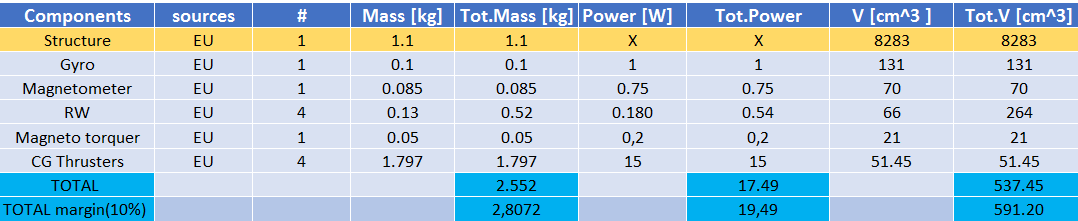
\includegraphics[scale=0.78]{table.PNG}


\caption{Budget}

\end{figure}
Please notice that in the mass,volume and power budget additional on board devices are not taken into consideration  such as: antennas,batteries,solar panels,.... and you name it. 
From the data available the evaluation of the inertia matrix referred to the principal axis is straightforward:
\begin{equation}
\mathbf{I}=
\begin{bmatrix}                   
0.218&0&0\\
0&0.166&0\\
0&0&0.082
\end{bmatrix} \ \ [kgm^2]
\end{equation}
\clearpage
\section{Model description}
\subsection{Assumptions and approximations:}
\subsubsection{Orbital mechanics:}



%\begin{table}[H]
%\centering
 %\begin{tabular}{|P{2cm}|P{2cm}|P{2cm}|P{2cm}|P{2cm}|P{2cm}|}

%\hline
% \rowcolor{gray}
%$\begin{matrix}
%a_{geo}\\ [km]
%\end{matrix} $ & $e_{geo}$ & $\begin{matrix}
%i_{geo}\\ [rad]
%\end{matrix}$ & $\begin{matrix}
%\omega_{geo}\\ [rad]
%\end{matrix}$&
%$\begin{matrix}
%\Omega_{geo}\\ [rad]
%\end{matrix}$ & $\begin{matrix}
%\theta_{geo}\\ [rad]
%\end{matrix}$\\
%\hhline{|=|=|=|=|=|=|}
%42164 & 0 & 0 & 0 & 0 & 0\\
%\hline

%\end{tabular}
%\end{table}
\begin{figure} [H]
\centering 
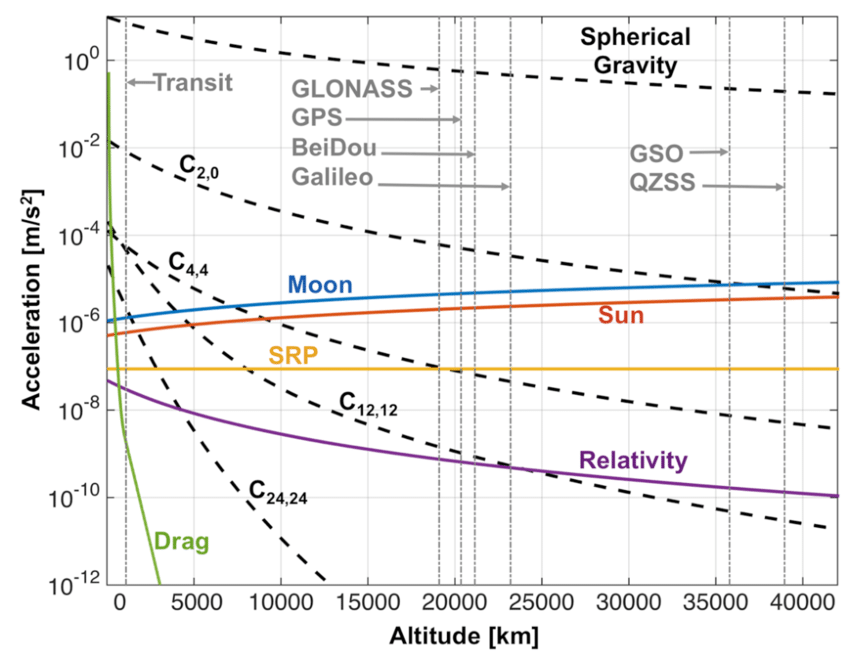
\includegraphics[scale=0.3]{Perturbations.png}
\caption{ importance of orbital perturbations
\cite{perturbations}}
\end{figure}
The satellite under analysis is set on a GEO orbit.  For the the orbital mechanics , as to ease the solution process, the motion is modeled without any kind of perturbation due to : J2,SRP,Magnetic disturbance  and so on and so forth. This is certainly a coarse approximation, since in reality the orbit is sensitive to all of them.On the other hand there is no presence of air in GEO orbit, so drag forces can be completely discarded. This picture summarizes the all effects said before:

\subsubsection{Satellite dynamics and attitude:}
\begin{figure} [H]
\centering 
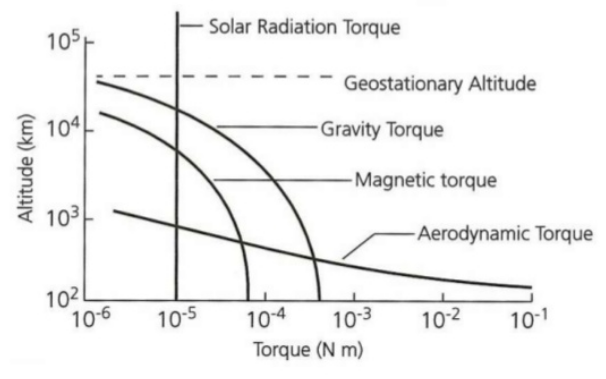
\includegraphics[scale=0.70]{torquessss.PNG}
\caption{ disturbance torques
\cite{perturbationss}}
\end{figure}
The aim is to study the local dynamics and to develop for this one control algorithms . In addition, aside from the de-tumbling which occurs in a small time frame, for slew and Sun pointing the perturbations quoted before are all developed with different models in the following section. It is worth noting that the spacecraft is treated as rigid body, \textit{(no vibrations or continuous mechanics involved)}. 




\subsubsection{Sun position:}
\begin{minipage}{.5\textwidth}
\begin{figure} [H]
\centering 
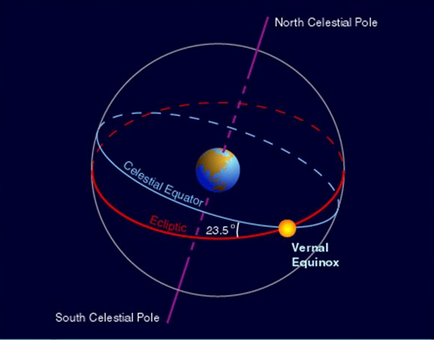
\includegraphics[scale=0.79]{ecliptic.PNG}
\caption{ Sun position
\cite{ecliptic}}
\end{figure}
\end{minipage}
\begin{minipage}{.5\textwidth}
\begin{equation}
r_{Sun}= 149600000 \ [Km]
\end{equation}
\begin{equation}
\omega_{Sun}=\frac{2 \pi}{365.25 \cdot 24 \cdot 3600 }=1.99 \cdot 10^{-7} \ \left[ \frac{rad}{s} \right] 
\end{equation}
\end{minipage}\\\\
Since the inertial reference frame is located in the Earth equatorial reference frame, the position of the Sun will change over time , instead the earth will remain fixed. As first approximation the orbit described by the star is circular with constant angular velocity. Actually this is a good model because the eccentricity the Earth orbit is $ e=0.0167$, defining  a nearly circular orbit.
\subsubsection{Cold-Gas thruster:}
Here the main assumption is that the satellite  has a constant mass through the detumbling , when the Cold-Gas thruster operates.A rough approximation   the mass flow rate is given by:
\begin{equation}
    \dot{m_p}=\frac{2F}{Ispg_E}=3.4\cdot10^{-5} \frac{Kg}{s}
\end{equation}
 Considering a detumbling time of 90s, the total expelled mass is :
 \begin{equation}
     m_{expelled}=90\cdot3.4\cdot10^{-5}=3\cdot10^{-3} \ \ Kg.
 \end{equation}
\subsection{Mathematical Model:}
\subsubsection{Reference frame:}
\begin{minipage}{.5\textwidth}
\begin{figure} [H]
\centering 
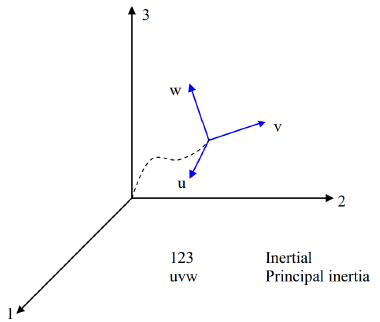
\includegraphics[scale=0.9]{reference_frame.PNG}
\caption{ Inertial and body reference frame
\cite{reference_frame}}
\end{figure}
\end{minipage}
\begin{minipage}{.5\textwidth}
There are different ways to define the attitude of a spacecraft. The one selected for this project is through the direct cosine matrices. Each axis of a reference frame is determined by three components of its unit direction vector. 
\begin{equation}
\mathbf{A}=\begin{bmatrix}
u_1 & u_2 & u_3 \\
v_1& v_2 & v_3 \\
w_1 & w_2 & w_3 \\
\end{bmatrix}
\end{equation}
This matrix allows to switch the representation of a vector from one reference to another one in this way:
\begin{equation}
\mathbf{a_{uvw}} = \mathbf{A} \mathbf{a_{123}}
\end{equation}
\end{minipage}
\\\\
The transformation does not affect both the magnitude and the relative orientation of the unit vectors. These constraints are expressed by the following properties :
\begin{equation}
\mathbf{A}\mathbf{A^T}=\mathbf{I} \ \ \ \ \ \ \ \ and \ \ \ \ \ \ \ \  det(\mathbf{A})=1
\end{equation}

In particular the inertial reference frame \textit{(represented by the Earth itself)} and the body one are identified by :\\
\begin{minipage}{.5\textwidth}
\begin{equation}
\mathbf{N}=\begin{bmatrix}
1 & 0 & 0 \\
0& 1 & 0 \\
0 & 0 & 1 \\
\end{bmatrix}
\end{equation}
\end{minipage}
\begin{minipage}{.5\textwidth}
\begin{equation}
\mathbf{B}=\mathbf{A_{B/N}}\mathbf{N}
\end{equation}
\end{minipage}
The matrix  \ $ \mathbf{A_{B/N}}$ will be evaluated at each time step , based on the relative orientation of the spacecraft  with respect to the Earth.

\subsubsection{Euler Equation:}
The system of differential equations outlining the dynamics of the satellite, are the so called Euler equations:

\begin{equation}
\begin{cases}
\dot{\omega}_x=\displaystyle\frac{I_y-I_z}{I_x}\omega_y \omega_z + \displaystyle\frac{M_x}{I_x} \\\\
\dot{\omega}_y=\displaystyle\frac{I_z-I_x}{I_y}\omega_z \omega_x + \displaystyle\frac{M_y}{I_y} \\\\
\dot{\omega}_z=\displaystyle\frac{I_x-I_y}{I_z}\omega_x \omega_y + \displaystyle\frac{M_z}{I_z} 
\end{cases}
\end{equation}
\\ Please notice that $ M_x,M_y$ and $ M_z$ comprises both the disturbances and the control actuation.
\subsubsection{Attitude:}
The ideal attitude matrix is governed by this  system of differential equations:
\begin{equation}
\mathbf{\dot{A}_{B/N}}=-[\boldsymbol{\omega}^\wedge ]\mathbf{{A}_{B/N}}
\end{equation}
Despite this relation an instrument on board for detecting the attitude matrix is always needed.
The attitude matrix along with the integration looses the orthonormal properties  . There is an iterative procedure to retrieve these features :
\begin{equation}
\mathbf{A_{k+1}}=\frac{3}{2}\mathbf{A_k}-\mathbf{A_k}\mathbf{A_k}^T\mathbf{A_k}\frac{1}{2}
\end{equation}

\subsubsection{Gravity Gradient torque:}
\begin{minipage}{.5\textwidth}
\begin{figure} [H]
\centering 
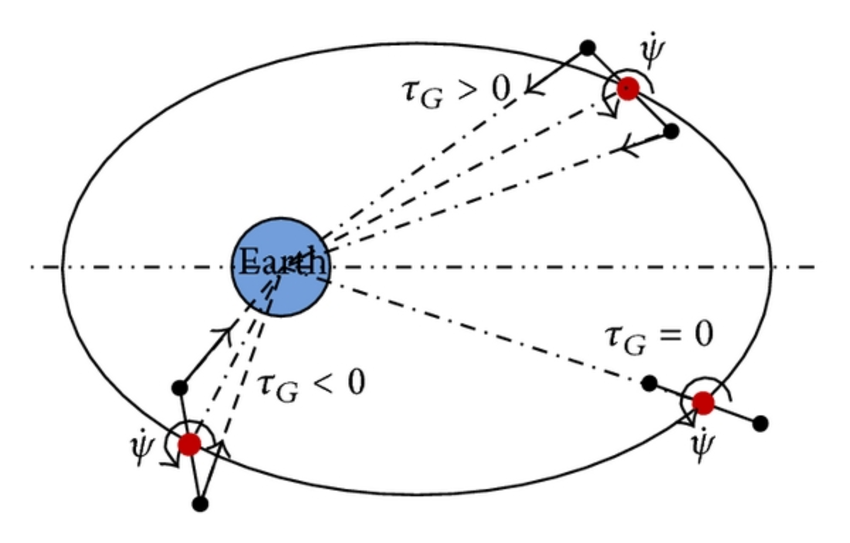
\includegraphics[scale=1]{GG.png}
\caption{ Gravity Gradient Torque
\cite{GG}}
\end{figure}
\end{minipage}
\begin{minipage}{.5\textwidth}
The gravity field is not uniform,thus a torque could act on the satellite. This kind of perturbation is relevant for large satellites due to long time action.In its more generic definition the torque yielded by the elementary force $f$ acting on the infinitesimal mass $m$ is:
\begin{equation}
\mathbf{m_{GG}}=- \int_b  \mathbf{r} \times \frac{Gm_E}{|r+r_{sc}|^3}(\mathbf{r_{sc}}+\mathbf{r})dm
\label{gg}
\end{equation}
Where $\mathbf{r_{sc}}$ is the position vector of the center of mass and $r$ the one from the center of mass to any other point of the spacecraft.
\begin{equation}
r_{sc} >> r
\end{equation}

\end{minipage}\\\\\\
By making few steps \textit{(here not reported)} and evaluating all the terms under the integral sign, the \ref{gg} turns into:
\begin{equation}
\mathbf{m_{GG}}= \frac{Gm_E}{r_{sc}^3}\begin{bmatrix}
(I_z-I_y)c_2c_3\\
(I_x-I_z)c_1c_3\\
(I_y-I_x)c_1c_2
\end{bmatrix}
\end{equation}
$c_1,c_2$ and $c_3$ are the direction cosines of the radial direction in principal axes.
\subsubsection{SRP:}

\begin{figure} [H]
\centering 
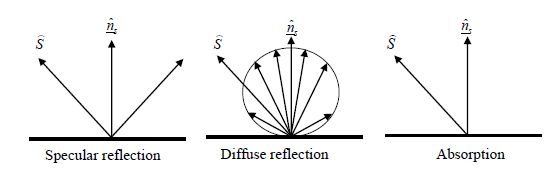
\includegraphics[scale=1]{SRP.PNG}
\caption{ reflection and absorption
\cite{SRP}}
\end{figure}


Solar radiation, illuminating the surface of a satellite, determines the presence of a pressure, leading to a torque around the center of mass of the satellite. The are 2 sources of this kind of phenomena : the Sun and the Earth. The former has usually a stronger effect and it can be stated to be constant around our planet.  The latter instead, resulted by reflection of the Sunlight is strongly dependent on the distance. The following table summarizes the typical values:\\
\begin{minipage}{.6\textwidth}
\begin{figure} [H]
\centering 
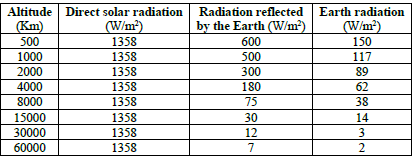
\includegraphics[scale=1.1]{SRP1.PNG}
\caption{ Typical values of  SRP 
\cite{SRP}}
\end{figure}
\end{minipage}
\begin{minipage}{.4\textwidth}
The pressure of the electromagnetic radiation can be computed as:
\begin{equation}
P=\frac{F_e}{c}
\end{equation}
$ F_e$ is the power per unit surface and $ c$ the speed of light. 
Part of the incident radiation is reflected part is absorbed .
\end{minipage}\\\\
As a result the exchange of forces are as follows:
\begin{equation}
\mathbf{f}=PA(\hat{\mathbf{s}}_b\cdot  \hat{\mathbf{n}}_s)[(1-\rho_s)\hat{\mathbf{s}}_b\dot +(2\rho_s(\hat{\mathbf{s}}_b\cdot  \hat{\mathbf{n}}_s)+\frac{2}{3}\rho_d )\hat{\mathbf{n}}_s]
\end{equation}
The knowledge or the attitude matrix $\mathbf{A_{B/N}}$ makes the calculation of the Sun position in the body frame easy:
\begin{equation}
\hat{\mathbf{s}}_b=\mathbf{A_{B/N}}\hat{\mathbf{s}}_N
\end{equation}
The satellite is shaped like a cuboid, whose principal axes are oriented as the normal vectors of the outer surfaces:

\begin{equation}
\hat{\mathbf{n}}_{s1}^b=\begin{bmatrix}
1&0&0
\end{bmatrix}
\ \ \ \ \ \ \ 
\hat{\mathbf{n}}_{s2}^b=\begin{bmatrix}
0&1&0
\end{bmatrix}
\ \ \ \ \ \ \
\hat{\mathbf{n}}_{s3}^b=\begin{bmatrix}
0&0&1
\end{bmatrix}
\end{equation}

\begin{equation}
\hat{\mathbf{n}}_{s4}^b=\begin{bmatrix}
-1&0&0
\end{bmatrix}
\ \ \ \ \ \ \ 
\hat{\mathbf{n}}_{s5}^b=\begin{bmatrix}
0&-1&0
\end{bmatrix}
\ \ \ \ \ \ \ 
\hat{\mathbf{n}}_{s6}^b=\begin{bmatrix}
0&0&-1
\end{bmatrix}
\end{equation}\
Last but not least the total torque acting on the satellite is now available:
\begin{equation}
\mathbf{t_{SRP}}=\begin{cases}
\sum_{i=1}^{n_{surfaces}} \mathbf{c_{pi}} \times \mathbf{f_i} \ \ \ \ \ if \ \ \ \ \ \hat{\mathbf{s}}_b \cdot  \hat{\mathbf{n}}_{s_i}^b \ > \ 0 \\
0 \ \ \ \ \ if \ \ \ \ \ \hat{\mathbf{s}}_b\cdot  \hat{\mathbf{n}}_{s_i}^b \ \leq\ 0 
\end{cases}
\end{equation}


\subsubsection{Magnetic disturbance:}
First of all before studying parasitic magnetic moment acting on the spacecraft, it is of paramount importance to derive the magnetic dipole  model for the Earth.This approximation is suitable for spacecrafts orbiting with an altitude greater than 7000km but lower than 10 Earth radii. In the inertial frame the vector of the  magnetic field $ \mathbf{b_N}$ is:\\
\begin{minipage}{.36\textwidth}
\begin{equation}
\mathbf{b_N}=\displaystyle\frac{R_E^3H_0}{r^3}[3({\mathbf{\hat{m}_E} }\cdot \mathbf{\hat{r}_{sc}}){\mathbf{\hat{r}_{sc}}}-{\mathbf{\hat{m}_E}}]
\end{equation}
\begin{equation}
H_0=\sqrt[]{(g_0^0)^2+(g_1^1)^2+(h_1^1)^2}
\end{equation}

\end{minipage}
\begin{minipage}{.64\textwidth}
\begin{figure} [H]
\centering 
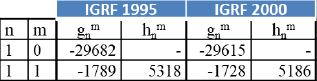
\includegraphics[scale=0.9]{coefficients.PNG}
\caption{ Gaussian coeff. in nT
\cite{coefficients}}
\end{figure}
\end{minipage}\\\\\\
 The versor along the dipole axis ${\mathbf{\hat{m}_E}}$ and the position one of the spacecraft ${\mathbf{\hat{r}_{sc}}}$  are:
\begin{equation}
\mathbf{\hat{m}_E}=\begin{bmatrix}sin(11.5 \degree)cos(\omega_Et)& sin(11.5 \degree)sin(\omega_Et) &cos(11.5 \degree)
\end{bmatrix}
\end{equation}
\begin{equation}
\mathbf{\hat{r}_{sc}}=\begin{bmatrix}
cos(\omega_Et) &sin(\omega_Et) &0
\end{bmatrix}
\end{equation}
Then the magnetic field in the body frame $\mathbf{b_B} $ is:
\begin{equation}
\mathbf{b_B}=\mathbf{A_{B/N}}\mathbf{b_N}
\end{equation}
 It can be measured by the magnetometer installed on board.
The interaction between the local magnetic field ad the flow of current generates a torque given by the formula :
\begin{equation}
\mathbf{t}_{mag_{dist}}=\mathbf{m_{sc}} \times \mathbf{b_B} 
\end{equation}
$ \mathbf{m_{sc}}$ is the residual  magnetic induction . The unit of measure of $ \mathbf{m_{sc}}$  can be stated as  $ Am^2$. In order to simulate the presence of $ \mathbf{m_{sc}}$ it is reasonable to adopt an average constant value , which expresses a worst case scenario:
\begin{equation}
\mathbf{m_{sc}} =\begin{bmatrix}

0.1&0.1&0.1
\end{bmatrix}^T \ \ \ [Am^2]
\end{equation}
\subsubsection{Gyro}
The gyroscopes are implemented on board to measure the angular velocities. The components of this device can be depicted by the image shown below:\\\\
\begin{minipage}{.5\textwidth}
\begin{figure} [H]
\centering 
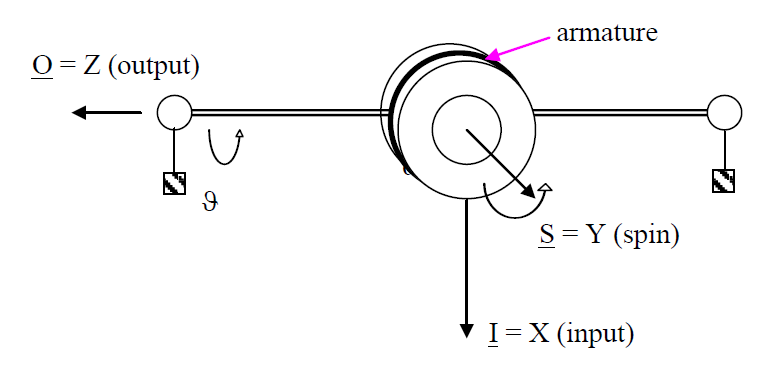
\includegraphics[scale=0.53]{Gyro1.PNG}
\caption{ Gyro
\cite{Gyro1}}
\end{figure}
\end{minipage}
\begin{minipage}{.5\textwidth}
The rotor rotates around the $\mathbf{S}$ axis and the support mechanism spins around the axis $\mathbf{O}$. The Euler equation of the system  are:
\begin{equation}
\begin{cases}
\omega_yJ_z\dot{\theta}-\overbrace{I_R}^{rotor}\omega_R(\omega_z+\dot{\theta})=M_x\\
I_R\dot{\omega_R}-\omega_xJ_z\dot{\theta}=M_y\\
\underbrace{J_z}_{rot+arm+sup} \ddot{\theta}+I_R\omega_R\omega_x=M_z
\end{cases}
\end{equation}
The first 2 equations provide the reaction forces and the third one the angular velocity $\omega_x$
\end{minipage}\\\\
As a steady state solution $\omega_x$ has the following value:
\begin{equation}
M_z=-k\theta -c\dot{\theta} \Longrightarrow
\omega_x=-\frac{k\bar{\theta}}{I_R\omega_R}
\end{equation}

\paragraph{Simple Gyro noise modeling:\\\\}
Every kind of measure is affected by noise , and the gyro copes with this issue as well:
\begin{equation}
\boldsymbol{\omega_{i}^m}=\boldsymbol{\omega_i+n+b}
\end{equation}
with:\\
\begin{minipage}{.5\textwidth}
\begin{equation}
\mathbf{n}=\sigma_n \mathbf{\zeta_n}
\label{n}
\end{equation}
\end{minipage}
\begin{minipage}{.5\textwidth}
\begin{equation}
\mathbf{\dot{b}}=\sigma_b \mathbf{\zeta_b}
\label{b_dot}
\end{equation}
\end{minipage}\\\\
$\sigma_n \mathbf{\zeta_n}$ and $\sigma_b \mathbf{\zeta_b}$  are defined as white Gaussian noise with zero mean value and respectively  standard deviation $\sigma_n$ and  $\sigma_b $ .The source of noise for the first one,known as angular random walk (ARW) , is strictly associated with thermo-mechanical noise.Concerning the second one, called RRW ( rate random walk), is related to the electric noise.To have the total noise contribution the \ref{b_dot} is integrated over time in all 3 components and summed with the \ref{n}.
\subsubsection{Magnetometer:}
A magnetometer  is an instrument that measures  the direction and strength of the magnetic field in the body frame.
This device is operated for the attitude determination by knowing at the same time $b_B$ and $b_N$, the local magnetic field and the inertial one.It is usually coupled with a Sun or an Earth horizon sensor, but not in this project. The output $\mathbf{A_{B/N}^*}$ is :\\\\
\begin{equation}
\mathbf{A_{B/N}^*}=\mathbf{A_{eps}}\mathbf{A_{B/N}}
\end{equation}
$\mathbf{A_{eps}}$ is the error matrix  and $\mathbf{A_{B/N}}$ the ideal attitude:
\begin{equation}
\mathbf{A_{eps}}=\begin{bmatrix}
cos(\epsilon)cos(\epsilon) & cos(\epsilon)sin(\epsilon)sin(\epsilon)+sin(\epsilon)cos(\epsilon)&-cos(\epsilon)sin(\epsilon)cos(\epsilon)+sin(\epsilon)sin(\epsilon)\\ 
    -sin(\epsilon)cos(\epsilon)&-sin(\epsilon)sin(\epsilon)sin(\epsilon)+cos(\epsilon)cos(\epsilon)&sin(\epsilon)sin(\epsilon)cos(\epsilon)+cos(\epsilon)sin(\epsilon)\\
  sin(\epsilon)& -cos(\epsilon)sin(\epsilon)& cos(\epsilon)cos(\epsilon)
\end{bmatrix}
\end{equation}
In a similar manner , as seen with the gyroscope , it exists a model for the noise contribution.
\begin{equation}
    \epsilon=p_{acc}\zeta_m
\end{equation}
\subsubsection{Magneto torquer:}
A magnetic torquer  is a satellite system for attitude control, detumbling, and stabilization built from electromagnetic coils. The magnetorquer creates a magnetic dipole that interfaces with an ambient magnetic field, usually Earth's, so that the counter-forces produced provide useful torque.
\begin{figure} [H]
\centering 
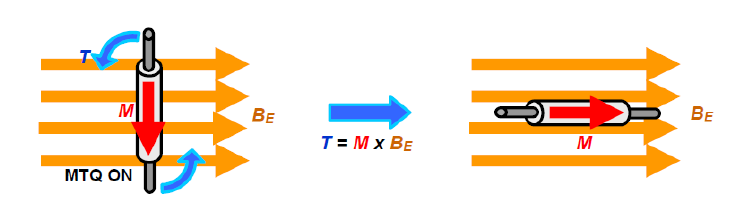
\includegraphics[scale=0.7]{Magneto_torquers1.PNG}
\caption{ Magneto torquer in action
\cite{MAgneto1}}
\end{figure}
The magnetic dipole $\mathbf{m_{MT}}$ of the rods, is proportional to current $\mathbf{i_{MT}}$ flowing  in it according to this relation:
\begin{equation}
\mathbf{m_{MT}}= c\mathbf{i_{MT}}
\end{equation}
 Next the torque is calculated:
\begin{equation}
\mathbf{t_{mag}}=\mathbf{m_{MT}}\times \mathbf{b_b}
\end{equation}
Where $\mathbf{b_b}$ is the Earth magnetic field vector in the body frame. Usually for de-tumbling there are  three-orthogonal magnetic torquers for 3-axis control. However, it is a sort of underactuated system because one of the rods can be aligned with the magnetic field direction without producing torque. On the other hand, while de-tumbling, the spacecraft is rotating and as consequence the direction of the magnetic field changes.\\\\
The parameter to play with , while implementing a  control law, is $\mathbf{m_{MT}}$. For the particular case under analysis see \ref{wwwww}
\subsubsection{Reaction wheels:}
A reaction wheel  is used primarily by spacecrafts for three axes attitude control, which doesn't require rockets or external applicators of torque. They provide a high pointing accuracy and are particularly useful when the spacecraft must be rotated by very small amounts, such as keeping a telescope pointed at a star.\\\\
\begin{minipage}{.5\textwidth}
\begin{figure} [H]
\centering 
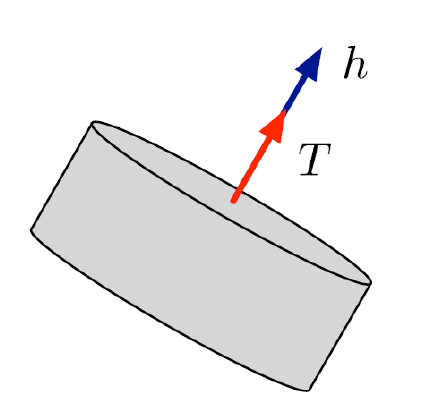
\includegraphics[scale=0.7]{RW1.PNG}
\caption{ Reaction wheel model
\cite{RW1}}
\end{figure}
\end{minipage}
\begin{minipage}{.5\textwidth}
Consider the Euler equations under the RW action:
\begin{equation}
\begin{cases}
\mathbf{I}\boldsymbol{\dot{\omega}}+\boldsymbol{{\omega}}\times\mathbf{I}\boldsymbol{\omega}+\boldsymbol{\omega}\times\mathbf{A}\mathbf{h_R}+\mathbf{A}\mathbf{\dot{h}}_R=0\\
\mathbf{u_c}=-\boldsymbol{\omega}\times\mathbf{Ah_R}-\mathbf{A\mathbf{\dot{h}}_R}\\
\boldsymbol{I_R\dot{\omega}_R}=\mathbf{\dot{h}_R}=\mathbf{t_R}
\end{cases}
\end{equation}
The control law can be extracted by this set of equations:
\begin{equation}
\mathbf{I}\boldsymbol{\dot{\omega}}+\boldsymbol{\dot{\omega}}\times\mathbf{I}\boldsymbol{\omega}=\mathbf{u_c}
\end{equation}
From any kind of control the requested $\mathbf{u_c}$ is known and the equation of interest becomes:
\begin{equation}
 \mathbf{\dot{h}_r}=\mathbf{A^*}(\mathbf{u_{c}}-\boldsymbol{\omega}\times \mathbf{A}\mathbf{h_r})
\end{equation}
\end{minipage}\\\\
In particular $\mathbf{A^*}$  is :
\begin{equation}
\mathbf{A^*}=\mathbf{A^T}(\mathbf{A}\mathbf{A^T})^{-1}
\end{equation}

\subsubsection{ Cold-Gas thrusters}
\begin{minipage}{.5\textwidth}

\begin{figure} [H]
\centering 
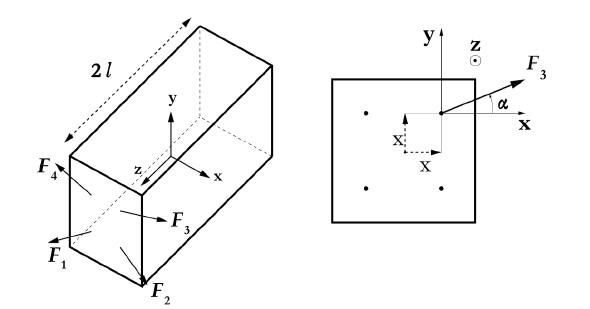
\includegraphics[scale=0.7]{disposition_thrusters.PNG}
\caption{ disposition of the thrusters
\cite{RW1}}
\end{figure}
\end{minipage}
\begin{minipage}{.5\textwidth}
The easiest way to provide a torque is to generate a set of forces not aligned with the center of mass.For Attitude control cold gas thrusters are very common and capable ,with few milli$-$Newton of applied force, to  do the job.The key point is to switch them  on and off on cue. They use a non reactive gas (He or N),stored at high pressure (approximately 30 MPa) . 
\end{minipage}
\\\\
Given the thruster configuration  in the figure, it corresponds a torque matrix computed by taking the cross product between the force of each thruster and the moment arm:\\
\begin{minipage}{.5 \textwidth}
\begin{figure} [H]
\centering 
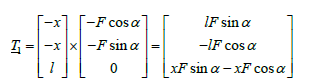
\includegraphics[scale=1]{Thrust_matr.PNG}
\end{figure}
\end{minipage}
\begin{minipage}{.5 \textwidth}
\ \ \ \ \ \ \ \ \ \ \ \ \ \  \ \ The relative configuration matrix is :
\begin{equation}
\mathbf{T}=
\begin{bmatrix}
\mathbf{T_1} & \mathbf{T_2} & \mathbf{T_3} & \mathbf{T_4}
\end{bmatrix}
\end{equation}
\end{minipage}
\clearpage
In more detail:
\begin{figure} [H]
\centering 
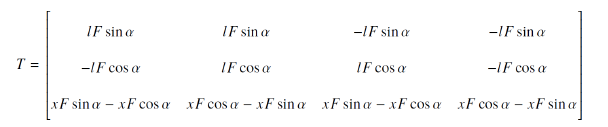
\includegraphics[scale=0.9]{TT_matr.PNG}
\end{figure}
\section{Control and determination Algorithms}
\subsection{De-tumbling}
\begin{figure} [H]
\centering 
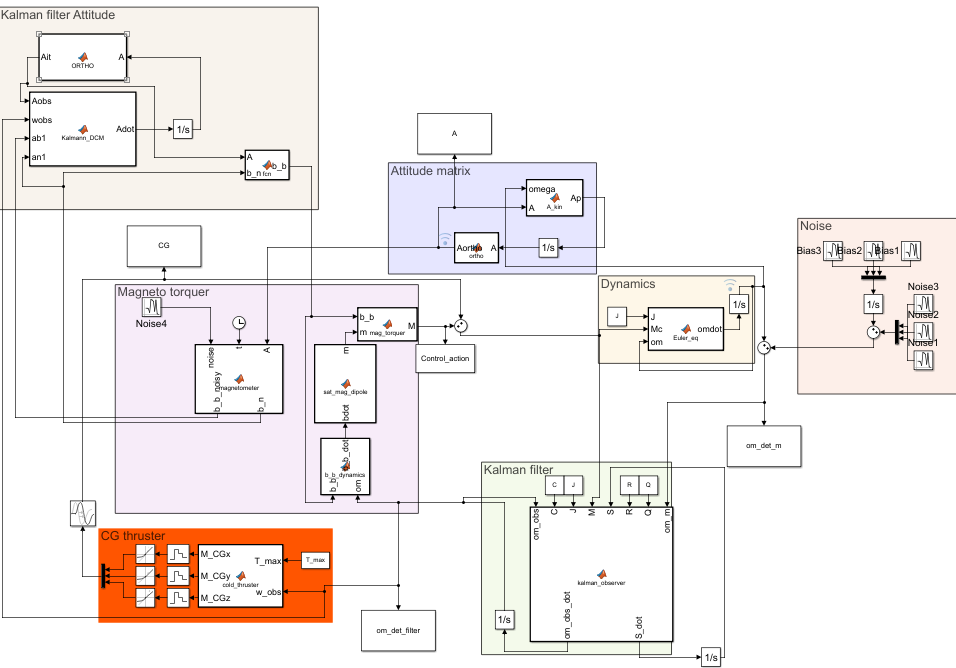
\includegraphics[scale=0.92]{detumbling.PNG}
\caption{ de-tumbling}
\end{figure}

\subsubsection{Kalman Filter:}
 Kalman filtering is an algorithm that uses a series of measurements observed over time, containing statistical noise and other inaccuracies, and produces estimates of unknown variables that tend to be more accurate than those based on a single measurement alone.It is useful to reconstruct the states of an observable dynamic system:\\\\
 \begin{minipage}{.5\textwidth}
\ \ \ \ \ Real system:\\
 \begin{equation}
 \begin{cases}
 \mathbf{\dot{x}}=\mathbf{f(x,u)+\overbrace{\mathbf{w}}^{disturbance}}\\ 
 \mathbf{\underbrace{\mathbf{y}}_{noisy\  signal}}=\mathbf{g(x,u)+\underbrace{\mathbf{v}}_{noise}}
 \end{cases}
 \end{equation}
 \end{minipage}
  \begin{minipage}{.5\textwidth}
\ \ \ \ reconstructed non linear system with noise filtering:\\
 \begin{equation}
 \begin{cases}
 \mathbf{\dot{\hat{x}}}=\mathbf{f(\hat{x},u)+L(y-\hat{y})}\\ 
\mathbf{\underbrace{ \mathbf{\hat{y}}}_{filtered \ signal}}=\mathbf{g(\hat{x})}

 \end{cases}
 \end{equation}
 \end{minipage}\\\\
 In the assigned problem the reconstructed state is done  by selecting $ \mathbf{C}$ as the identity matrix arbitrarily:
 \begin{equation}
 \begin{cases}
\dot{\omega}_{x_{obs}}=\displaystyle\frac{I_y-I_z}{I_x}\omega_{y_{obs}}\omega_{z_{obs}}+{l_{w_1}}+\displaystyle\frac{M_x}{I_x}\\\\
\dot{\omega}_{y_{obs}}=\displaystyle\frac{I_z-I_x}{I_y}\omega_{z_{obs}}\omega_{x_{obs}}+{l_{w_2}}+\displaystyle\frac{M_y}{I_y}\\\\
\dot{\omega}_{z_{obs}}=\displaystyle\frac{I_x-I_y}{I_z}\omega_{x_{obs}}\omega_{y_{obs}}+{l_{w_3}}+\displaystyle\frac{M_z}{I_z}
 \end{cases}
 with \ \ \mathbf{l}_w=\mathbf{L}(\boldsymbol{\omega-C\omega_{obs}})
 \end{equation}
 $ \mathbf{L}$ can be estimated through the solution of the following differential Riccati equation \cite{riccati}:\\\\
 \begin{minipage}{.5 \textwidth}
 \begin{equation}
    \mathbf{\dot{P} = PA^T + AP + Q - PC^T R^{-1} CP}
 \end{equation}
 \begin{equation}
     \mathbf{ L = PC^T R^{-1}}
 \end{equation}
 \begin{equation}
     \mathbf{A}=\begin{bmatrix}
     0 & K_x\omega_{z_{obs}} & K_x\omega_{y_{obs}} \\ K_y\omega_{z_{obs}}  & 0 & K_y\omega_{x_{obs}} \\ K_z\omega_{y_{obs}}  & K_z\omega_{x_{obs}}  & 0
     \end{bmatrix}= \left. \frac{\partial \mathbf{f}}{\partial\boldsymbol{w}} \right|_{\boldsymbol{\omega_{obs}}}
 \end{equation}
 \begin{equation}
    K_x = \frac{I_y-I_z}{I_x},  K_y = \frac{I_z-I_x}{I_y},  K_x = \frac{I_x-I_y}{I_z}
 \end{equation}
 \end{minipage}
  \begin{minipage}{.5 \textwidth}
 
 
 \begin{equation}
     \mathbf{ R }= \begin{bmatrix}
     \sigma_w^2 &0 &0\\
     0&   \sigma_w^2& 0 \\
     0& 0 & \sigma_w^2
     \end{bmatrix}
 \end{equation}
\begin{equation}
     \mathbf{ Q }= \begin{bmatrix}
     \sigma_v^2 &0 &0\\
     0&   \sigma_v^2& 0 \\
     0& 0 & \sigma_v^2
     \end{bmatrix}
\end{equation}
 \end{minipage}
 \subsubsection{Kalman Filter for DCM}
 The attitude matrix is reconstructed in this way:
 \begin{equation}
     \mathbf{\dot{\hat{A}}_{B/N}}=-[(\boldsymbol{\omega+\alpha)}^\wedge]\mathbf{\hat{A}_{B/N}}
 \end{equation}
 Where :
 \begin{equation}
     \boldsymbol{\alpha}=k_{DCM}(\mathbf{a_b \times \hat{A}_{B/N}a_n})
 \end{equation}
 The reconstruction of the state by means of the Kalman filter (\textit{as with the one for the dynamics}) is suitable for noise attenuation caused by the sensor measurement.
 \subsubsection{Control law for the Magneto Torquer:}\label{wwwww}
 From the theory a simple control law is derived for the magnetic torquers:
 \begin{equation}
 \mathbf{m}=-m_{max}sign(\mathbf{\dot{b}_b}) \ \ \ with \ 1\  magnetic \ torquer \ \ \ \mathbf{m}=-\begin{bmatrix}
 m_{max}sign(\mathbf{\dot{b}_{b1}})&0 &0
 \end{bmatrix}^T
 \end{equation}
 For a detumbling spacecraft $\dot{b}_b$ is
 \begin{equation}
 \mathbf{\dot{b}_b}=-[\boldsymbol{\omega]^\wedge}\mathbf{b_b}
 \end{equation}
 
  \subsubsection{Bang Bang Control:}
 Knowing the thruster configuration, it can be calculated the maximum torque delivered in each axis $T_{max_i}$. For example :
 \begin{equation}
     |{T_{max_1}}|=2lFsin(\alpha)
 \end{equation}
 As a consequence the maximum torque matrix is:
 \begin{equation}
   \mathbf{T_{max}} = \begin{bmatrix}
      |{T_{max_1}}|& 0 &0\\
      0&  |{T_{max_2}}| &0 \\
      0& 0 &  |{T_{max_3}}|
     \end{bmatrix}
 \end{equation}
 The Bang-Bang control requires the following definition:
 \begin{equation}
     \mathbf{u}=-\mathbf{T_{max}}sign(\boldsymbol{\omega})
 \end{equation}
 This formula is valid on with 12 or more thrusters , with only 4 thruster it is impossible to have the maximum torque simultaneously on the three axes. As matter of fact a suboptimal solution is found. A logic could be to activate the thrusters , which operate on the axis with the largest angular velocity.\\ For example :
 \begin{equation}
     \omega_{max}=\omega_x \Longrightarrow  \mathbf{u}=-\begin{bmatrix}
      |{T_{max_1}}|& 0 &0\\
      0&  0&0 \\
      0 & 0 & 0
     \end{bmatrix}
     sign(\mathbf{\boldsymbol{\omega}})
 \end{equation}
 Also possible rise ,fall times , MIB and delays of the actuator are taken into account by using the blocks in \textbf {Simulink Rate Limiter , zero order hold and transport delay} .
 To avoid chattering the actuation should be switched off when:
 \begin{equation}
     |\omega_{max}|< \epsilon_{Cold-Gas}
 \end{equation}
 \subsection{Slew Manoeuvre:} 
 \begin{figure} [H]
\centering 
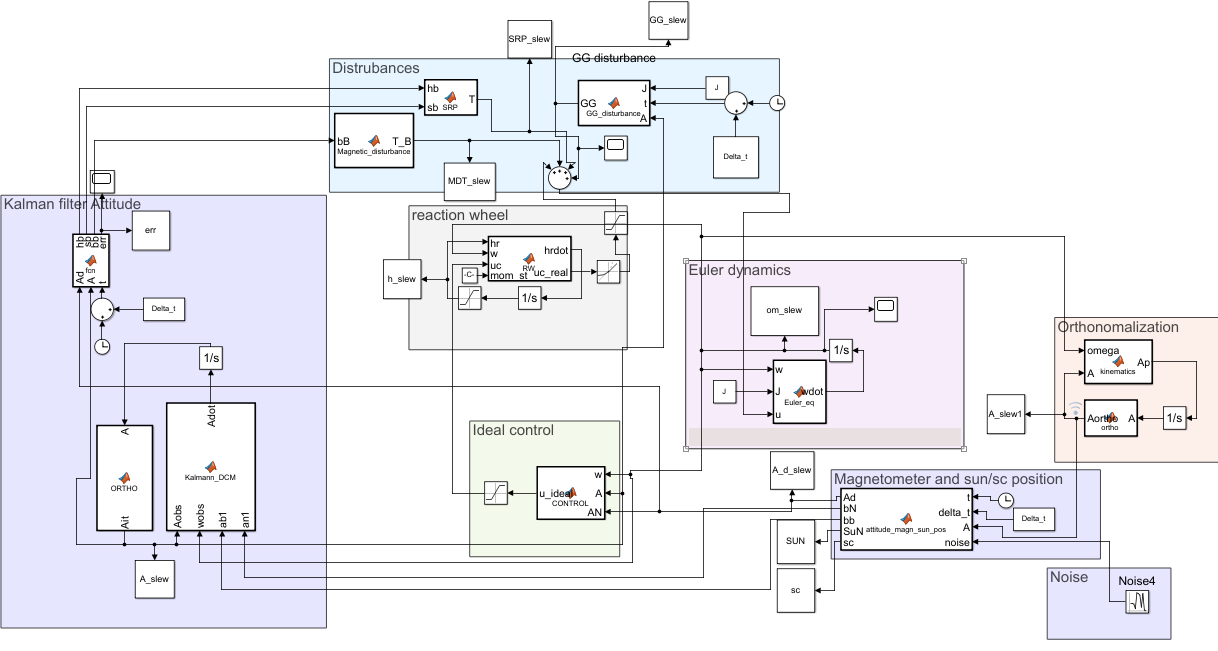
\includegraphics[scale=0.68]{slew.PNG}
\caption{ Slew Manoeuvre}

\end{figure}
 \subsubsection{Sun Pointing:} \label{sun}
 The main goal of the Cubesat is to rotate along its axis for an alignment with the Sun, that as first approximation has a fixed position in the space during the slew manoeuvre.Therefore to satisfy this requirement a desired attitude matrix $ \mathbf{A_d}  $ is built in this way at $t^*=T_{det}$ :
  \begin{equation}
     \mathbf{r_{sc}}=r_{sc}\begin{bmatrix}
     cos(n_et)&sin(n_et)&0
     \end{bmatrix}
 \end{equation}
 \begin{equation}
     \mathbf{r_{sun}}=r_{sun}\begin{bmatrix}
   cos(n_{sun}t+B)& sin(n_{sun}t+B)cos(23.45)& sin(n+B)sin(23.45)
     \end{bmatrix}    
 \end{equation}
 \begin{minipage}{.5\textwidth}
 \begin{equation}
\mathbf{x_1}=\frac{\mathbf{r_{sun}}(t^*)-\mathbf{r_{sc}}(t^*)}{||\mathbf{r_{sun}}(t^*)-\mathbf{r_{sc}}(t^*)||}
 \end{equation}
  \begin{equation}
 \mathbf{x_3}=\frac{(\mathbf{r_{sun}}(t^*)-\mathbf{r_{sc}}(t^*)) \times (\mathbf{v_{sun}}(t^*)-\mathbf{v_{sc}}(t^*))}{||(\mathbf{r_{sun}}(t^*)-\mathbf{r_{sc}}(t^*)) \times (\mathbf{v_{sun}}(t^*)-\mathbf{v_{sc}}(t^*))||}
 \end{equation}
 \end{minipage}
 \begin{minipage}{.5\textwidth}
  \begin{equation}
 \mathbf{x_2}=\frac{\mathbf{x_3}\times\mathbf{x_1}}{||\mathbf{x_3}\times\mathbf{x_1}||}
 \end{equation}
 \begin{equation}
 \mathbf{A_d}=\begin{bmatrix}
 \mathbf{x_1}\\
  \mathbf{x_2}\\
 \mathbf{x_3}
 \end{bmatrix}
 \end{equation}
 \end{minipage}\\\\
  $ \mathbf{x_1} $is chosen as pointing axis because related to the direction with the maximum inertia, good for stability purposes.The quantification of the error between the desired attitude and the real one can be determined estimated as
  \begin{equation}
      err=trace(\mathbf{I}-\mathbf{A_{B/N}A_d^T})
  \end{equation}
  \subsubsection{Ideal Control:}\label{control}
  The ideal control tries to figure out  which is the correct value of torque that the reaction wheels need to grant.
  The expression is \label{erri}:\\\\
  \begin{minipage}{.5\textwidth}
  \begin{equation}
  \mathbf{u_{c_{ideal}}}=-k_1\boldsymbol{\omega_e}-\mathbf{e}
  \end{equation}
  \begin{equation}
  \boldsymbol{\omega_e}=\boldsymbol{\omega}
  \end{equation}
  \end{minipage}
  \begin{minipage}{.5\textwidth}
  \begin{equation}
    \mathbf{A_e}=\mathbf{A_{B/N}}\mathbf{A_d}
  \end{equation}
    \begin{equation}
  \mathbf{e}=k_2(\mathbf{A_e}^T-\mathbf{A_e})^{V}
  \end{equation}
  \end{minipage}
  \subsubsection{Real Control:}\label{real}
  In conclusion the ideal control becomes an input for the reaction wheel dynamics:
  \begin{equation}
  \mathbf{\dot{h}_r}=-\mathbf{A^*}(\mathbf{u_{c_{ideal}}}+\boldsymbol{\omega}\times \mathbf{A}\mathbf{h_r})
  \end{equation}
  \begin{equation}
      \mathbf{u_{c_{real}}}=-\boldsymbol{\omega}\times\mathbf{A h_r}-\mathbf{A\dot{h_r}};
  \end{equation}
  Bear in mind that as for the Cold-Gas thruster case , a \textbf{rate limiter} is set for the variation of the torque in time and a \textbf{a limiter} for the maximum momentum storage.In case of saturation a de-saturation procedure for the reaction wheels is necessary. for example:
  \begin{equation}
     \mathbf{\dot{h}_r}=-Tsign( \mathbf{{h}_r})
  \end{equation}
  
   A decreasing value in time of the angular momentum of the RW yields undesired torques on the satellite. As a consequence, the control torque required for attitude stabilization can no longer be generated by the wheels. To prevent this phenomenon, the momentum of the reaction wheels has to be rapidly unloaded by magnetic torquers and/or thrusters.
  \subsection{Tracking}
  The Simulink file is equal to the slew one apart from minor changes due to control actuation laws.
  \subsubsection{Pointing}
  The procedure is the same as seen in \ref{sun}, with a difference: the time is no more fixed so $\mathbf{A_d}$ will evolve over time.
  \subsubsection{Ideal control:}
    Here  the control law, compared to the Slew case, is transformed in a more complicated formulation because in presence of a time variant attitude an. In its more general formulation the relation  is:
    \begin{equation}
        \mathbf{u_{c_{ideal}}} =-k1\boldsymbol{\omega_e}-k_2(\mathbf{A_e}^T-\mathbf{A_e})^{V}+\boldsymbol{J\omega}\times\boldsymbol{\omega+J}(\boldsymbol{A_e\dot{\omega}_d-[\omega_e^{\wedge}] A_e\omega_d})
    \end{equation}
    In the event that  the frame evolves slowly in time, a reduced version is proposed:
     \begin{equation}
        \mathbf{u_{c_{ideal}}} =-k1\boldsymbol{\omega_e}-k_2(\mathbf{A_e}^T-\mathbf{A_e})^{V}+\boldsymbol{J\omega}\times\boldsymbol{\omega}
    \end{equation}
Definition of the involved variable:\\
\begin{minipage}{.5 \textwidth}
\begin{equation}
-\mathbf{\dot{A}_dA_d^T}  = [\boldsymbol{\omega_d}^{\wedge}]=\boldsymbol{\Omega}
\end{equation}
\begin{equation}
\boldsymbol{\omega_d}=\begin{bmatrix}
-\boldsymbol{\Omega}(2,3)& \boldsymbol{\Omega}(1,3) &-\boldsymbol{\Omega}(1,2)
\end{bmatrix}^T
\end{equation}
\end{minipage}
\begin{minipage}{.5 \textwidth}
\begin{equation}
      \mathbf{A_e}=\mathbf{A_{B/N}}\mathbf{A_d}
\end{equation}
\begin{equation}
    \boldsymbol{\omega_e}=\boldsymbol{\omega}-\mathbf{A_e}\boldsymbol{\omega_d}
\end{equation}

\end{minipage}\\\\\\
The following passages for the real control are the same as \ref{real}
\clearpage
\section{Results}\label{results}
\subsection{Detumbling}
\begin{minipage}{0.5\textwidth}
\begin{figure} [H]
\centering 
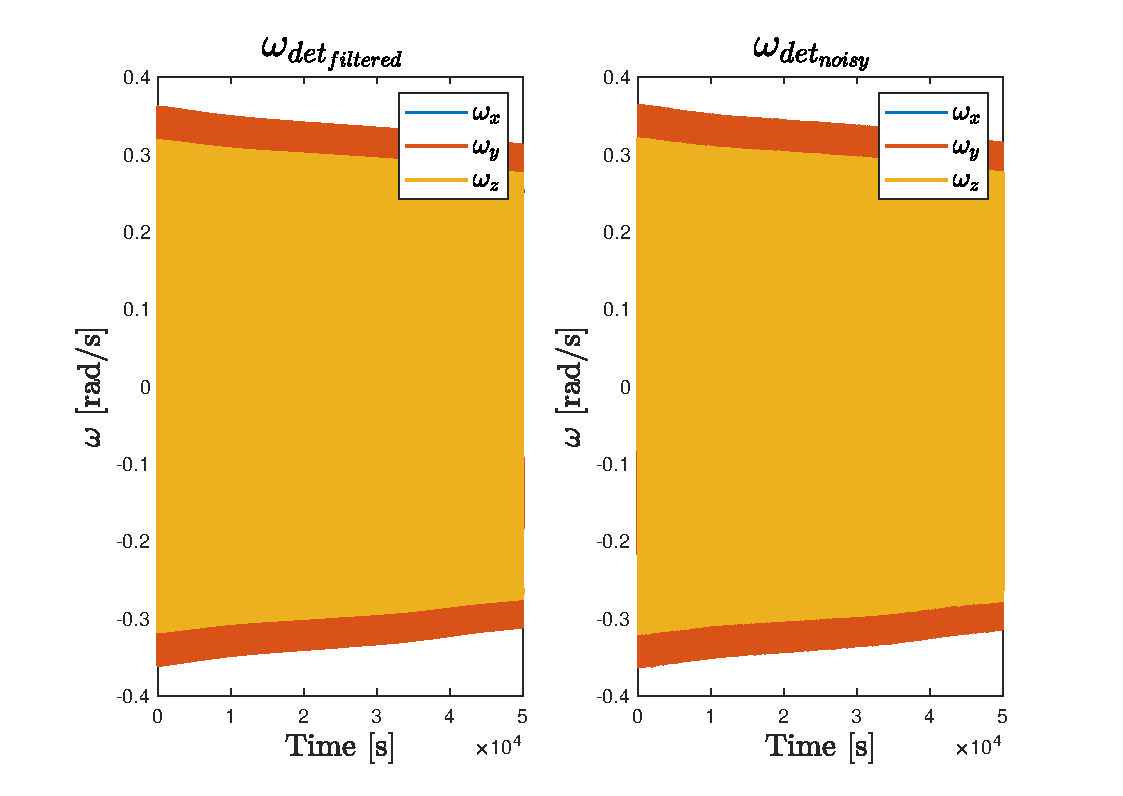
\includegraphics[scale=0.5]{w_magneto.eps}
\caption{ $\omega_{detumbling}$ with  only  magneto  torquers}

\end{figure}
\end{minipage}
\begin{minipage}{0.5\textwidth}
 \begin{figure} [H]
\centering 
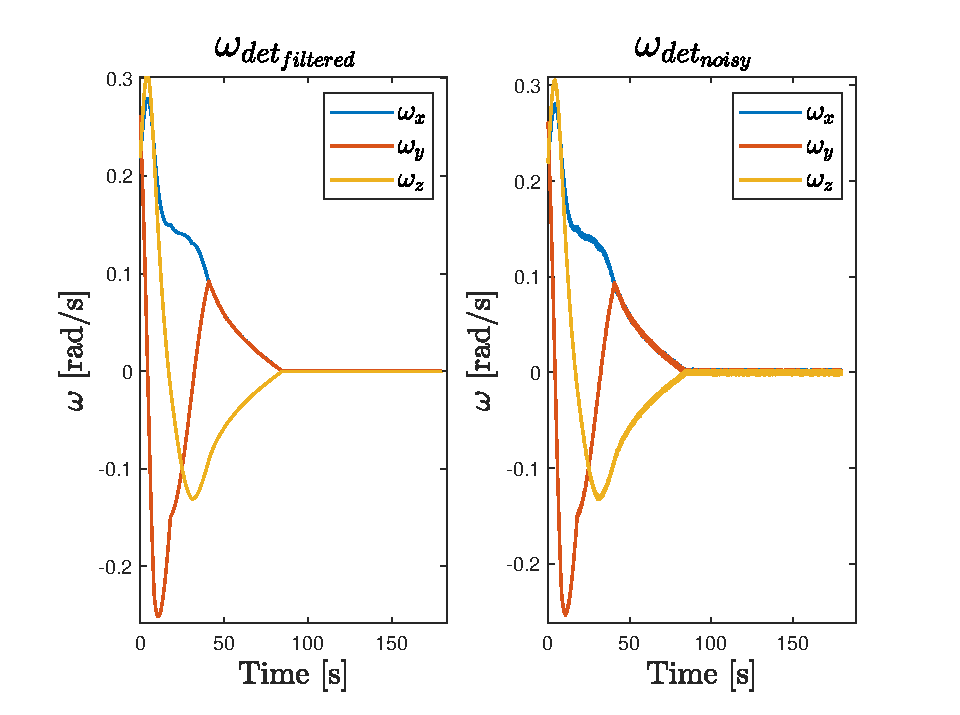
\includegraphics[scale=0.6]{w_det_cold_gas.eps}
\caption{ $\omega_{detumbling}$}
\label{CG}
\end{figure}
\end{minipage}\\\
 
In a GEO orbit the magnetic field of the Earth is so weak that the time required to de-tumble a 6U Cubesat is more than 50000 s, making the control actuation useless. This is the reason why Cold-Gas thrusters are introduced as part of the equipment.
First of all the improvement thanks to the installation of 4 Cold-Gas thrutsers is noticeable , compared to the previous solution , is able to bring to rest the satellite in less than 100 s. Secondly on the left hand side of \ref{CG} there is the reconstructed $\omega$ and on the right the one measured by the gyro. The Kalman filter combines the ability to follow the input signal  with filtering high frequencing oscillation due to noise.\\\\
\begin{minipage}{.5 \textwidth}
\begin{figure} [H]
\centering 
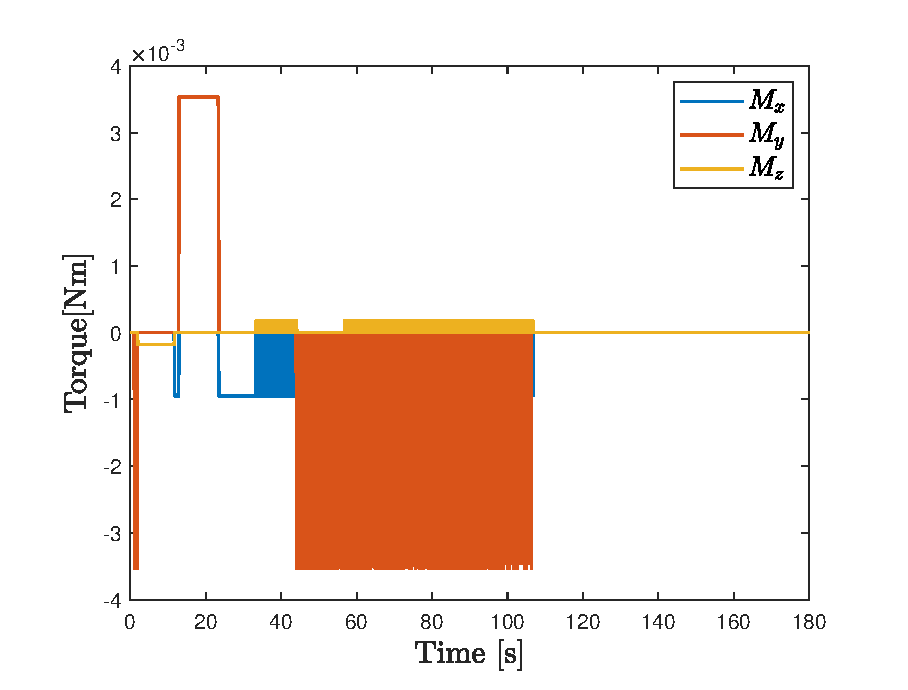
\includegraphics[scale=0.6]{CGT.eps}
\caption{ Cold-Gas thruster torque}
\label{cgt}
\end{figure}
\end{minipage}
\begin{minipage}{.5 \textwidth}
\begin{figure} [H]
\centering 
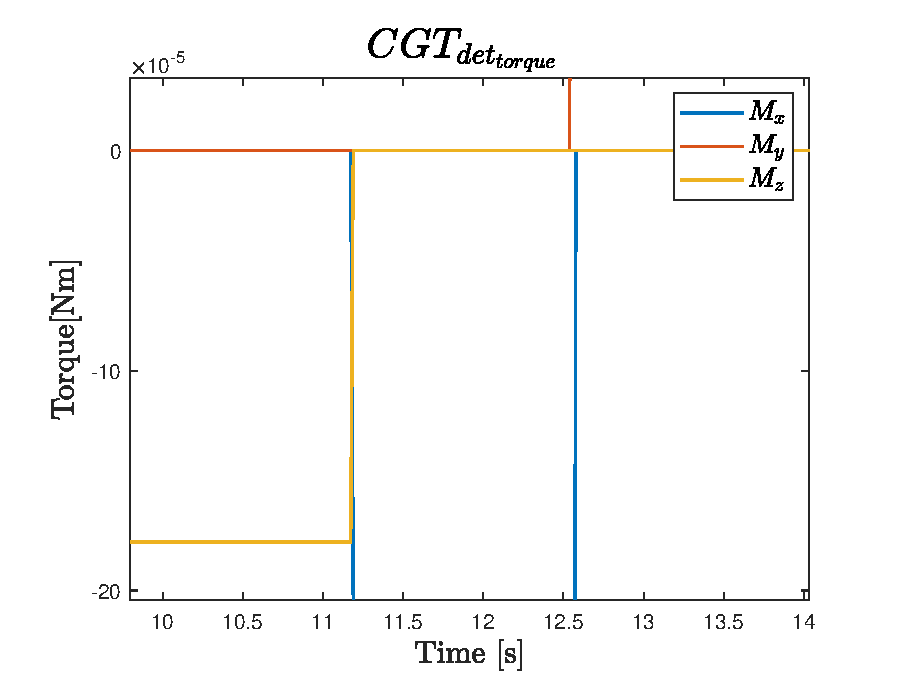
\includegraphics[scale=0.6]{zoom.eps}
\caption{ zoom of the Cold-Gas thruster torque}
\label{cgtt}
\end{figure}
\end{minipage}\\\\
The \ref{cgt} represents the evolution in time of the torque granted by the Cold-Gas thruster. From this figure it is understandable the functioning of the modified bang-bang control law. The torque is active on the different axes whenever the angular velocity is maximum. Between 40s to 100s, since the various components of $\boldsymbol{\omega}$ are almost equal in magnitude, there are a lot of firings. Furthermore after the de-tumbling the thrusters are not ignited any more in order to avoid chattering .The \ref{cgtt} is a zoom of the left hand side figure. Fall and rise time make not instantaneous the transition between on and off of  as predicted by the real model . 
\subsection{Slew Manoeuvre}
\begin{minipage}{.48 \textwidth}
\begin{figure} [H]
\centering 
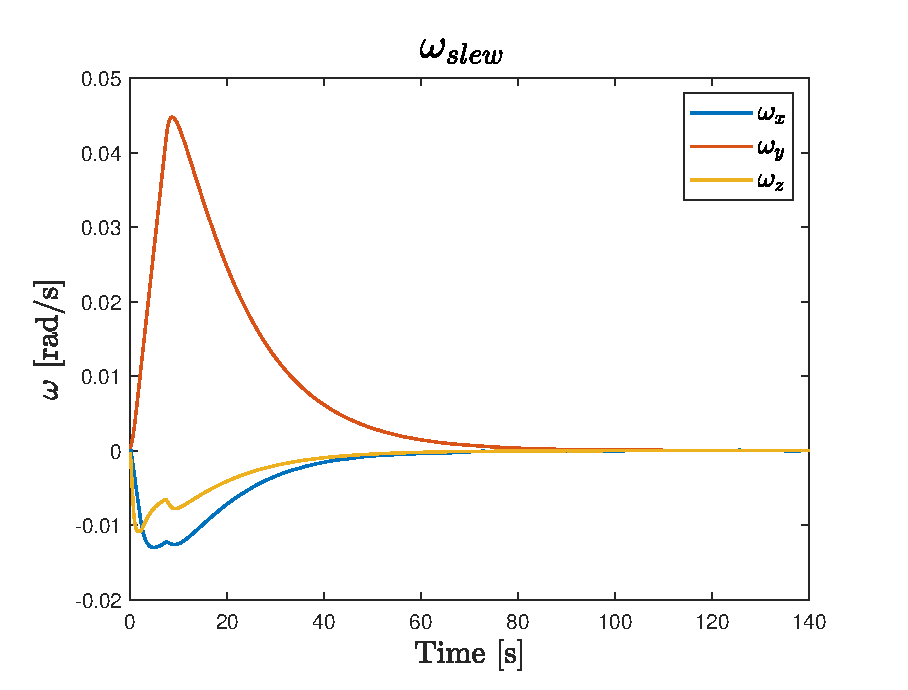
\includegraphics[scale=0.6]{w_slew.eps}
\caption{ $\omega_{slew}$}
\end{figure}
\end{minipage}
\begin{minipage}{.52 \textwidth}
\begin{figure} [H]
\centering 
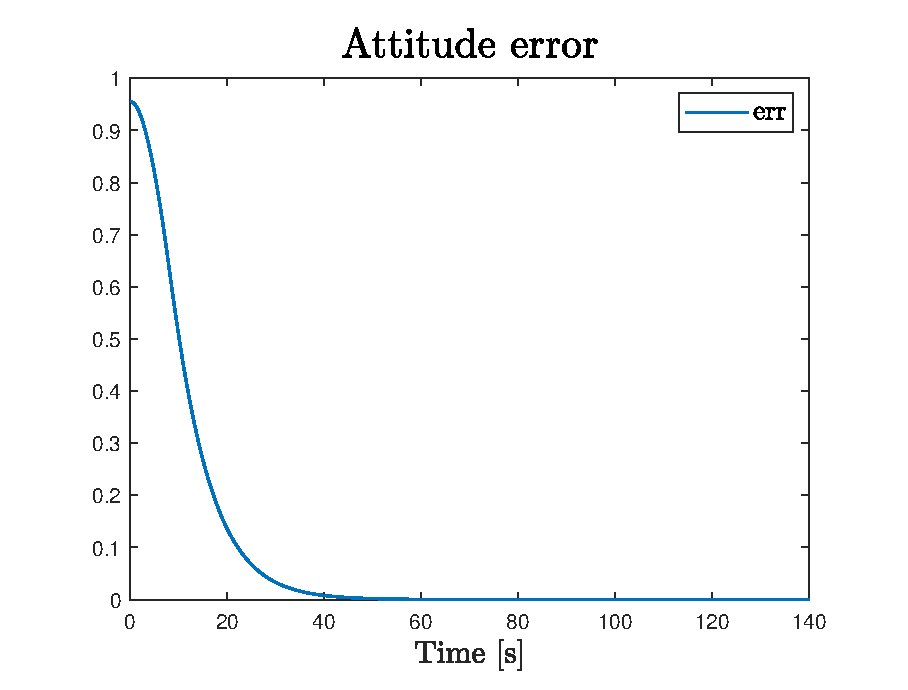
\includegraphics[scale=0.6]{A_err_slew.eps}
\caption{ error}
\label{err}
\end{figure}
\end{minipage}\\\\

The goal of the Slew is to perform a rest to rest manoeuvre. It has to steer the axes according to the position of the Sun, which is assumed to be fixed in time in this short time frame. After a transient of 70$-$ 80s it is capable of reaching the desired attitude.The formula used for \ref{err} is explained in \ref{erri}\\
\begin{minipage}{.45\textwidth}
\begin{figure} [H]
\centering 
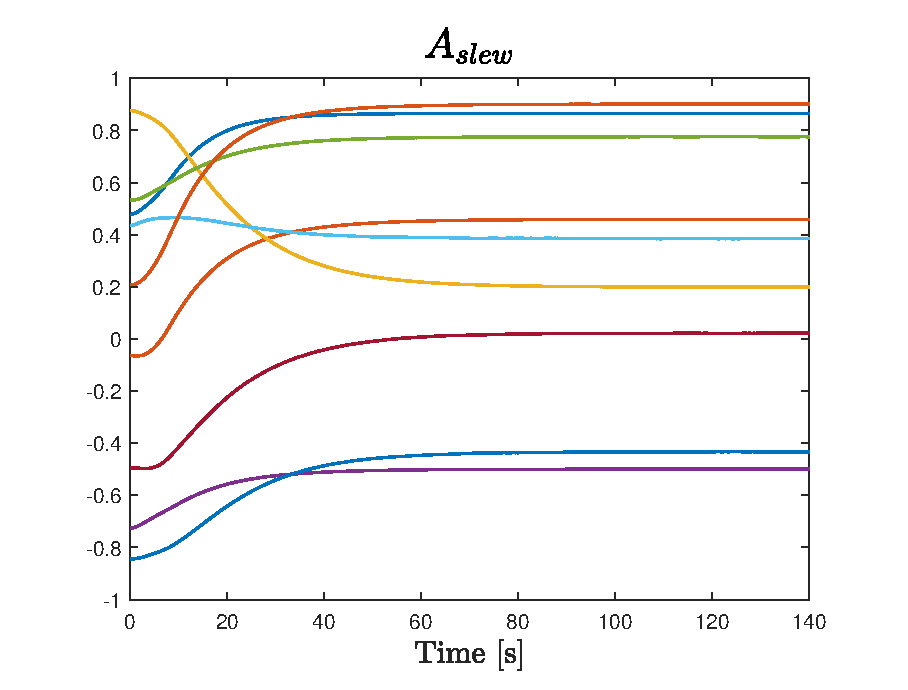
\includegraphics[scale=0.55]{A_slew_s.eps}
\caption{  filtered attitude matrix }
\label{as}
\end{figure}
\end{minipage}
\begin{minipage}{.55\textwidth}

\begin{figure} [H]
\centering 
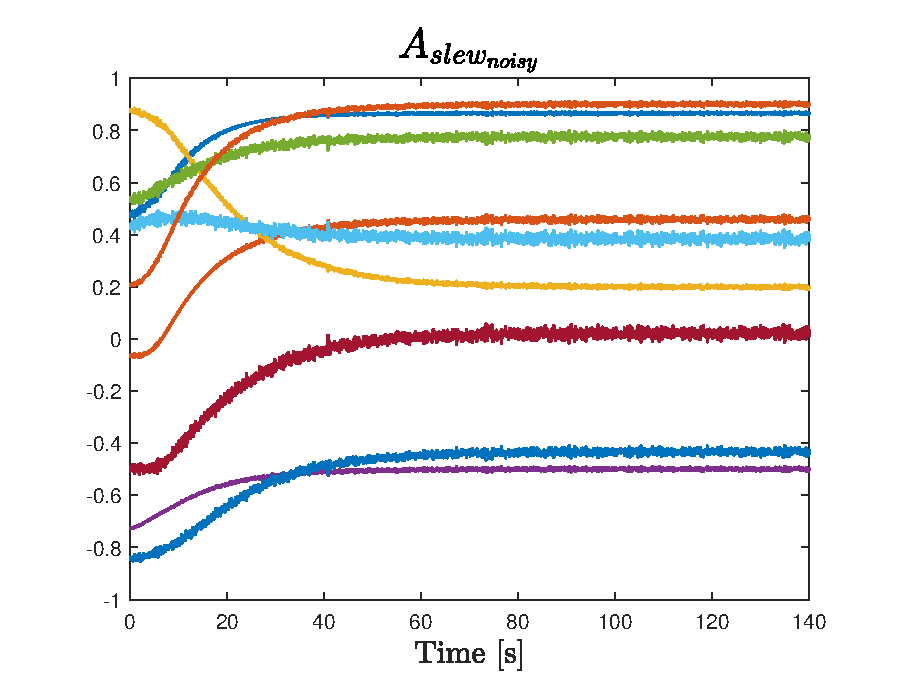
\includegraphics[scale=0.55]{A_slew_n.eps}
\caption{ Noisy attitude matrix }
\label{asn}
\end{figure}
\end{minipage}\\\\
The \ref{as} and \ref{asn} show the importance of having a Kalman filter also for the attitude reconstruction. All the high frequency components associated  to the magnetometer measurements are damped out through a suitable integral action. Similar results are derived  in tracking.



\begin{minipage}{.45\textwidth}
\begin{figure} [H]
\centering 
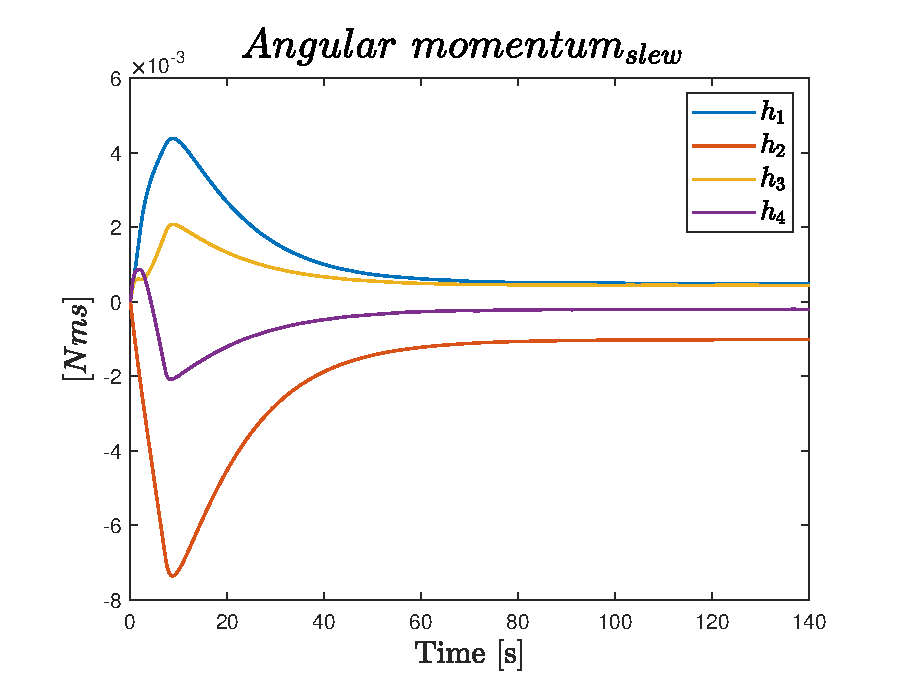
\includegraphics[scale=0.55]{ang_mom_slew.eps}
\caption{ angular momentum for the 4 RW}
\end{figure}
\end{minipage}
\begin{minipage}{.55\textwidth}
\label{rwrr}
\begin{figure} [H]
\centering 
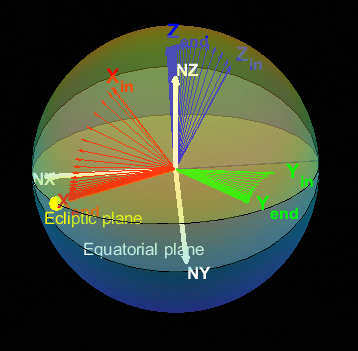
\includegraphics[scale=0.9]{SPHERE_SLEW.PNG}
\caption{ $3_d$ motion}
\label{3d_motion}
\end{figure}
\end{minipage}\\
The \ref{rwrr} stands for the evolution in time of the angular momentum related to the 4 RW. None of them reach the saturation condition, but at the end there is a residual angular momentum.The \ref{3d_motion} represents the evolution in time of the inertial principal axes during the slew manoeuvre. The yellow spot is the Sun position.\\\\\\

\begin{minipage}{.55 \textwidth}
\begin{figure} [H]
\centering 
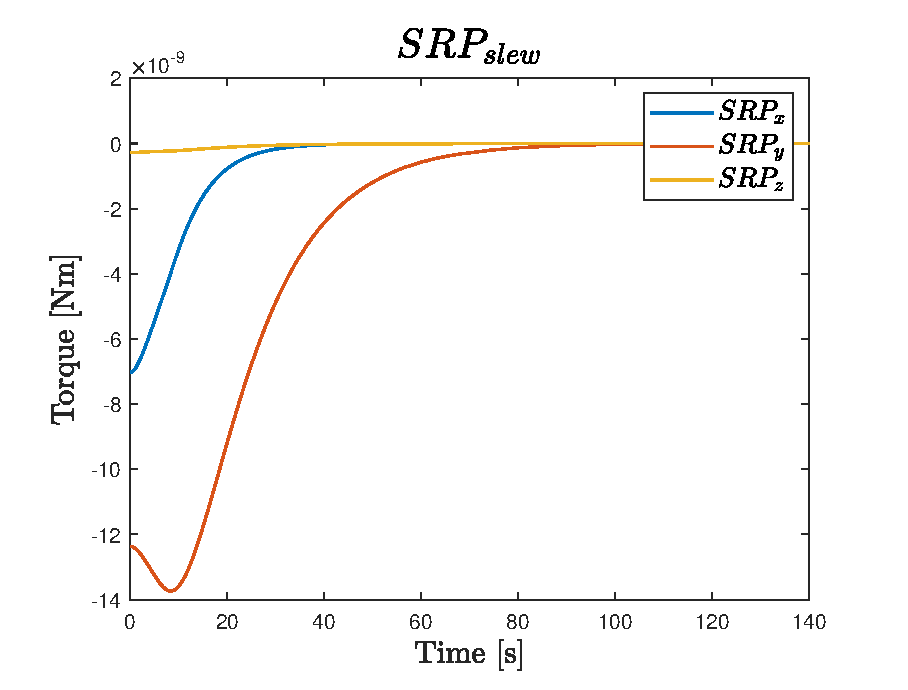
\includegraphics[scale=0.5]{SRP_slew.eps}
\caption{all the disturbances}
\end{figure}
\end{minipage}
\begin{minipage}{.45 \textwidth}
\begin{figure} [H]
\centering 
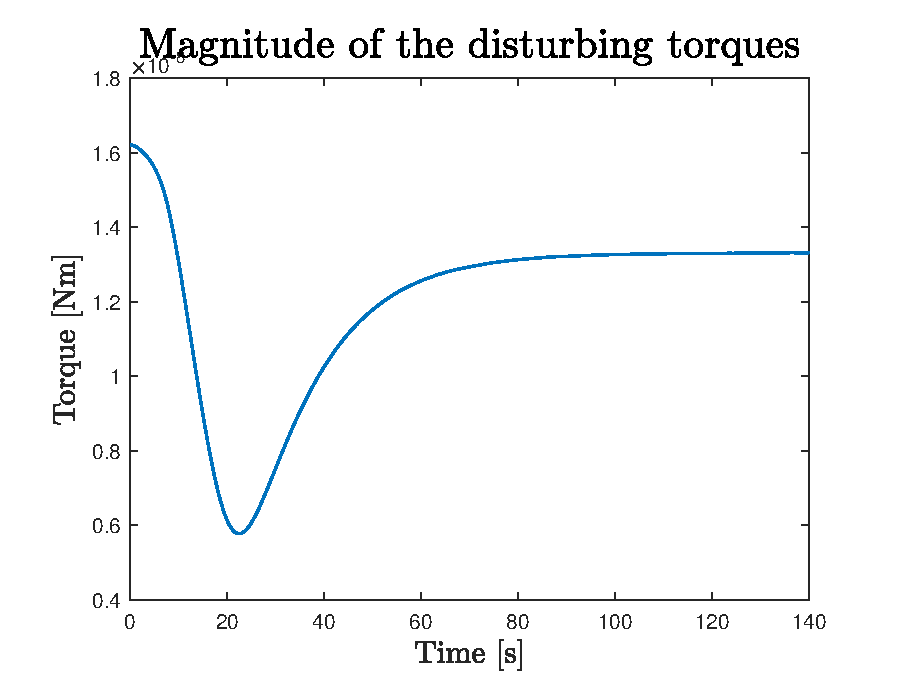
\includegraphics[scale=0.5]{magnitude.eps}
\caption{magnitude of the disturbances}
\end{figure}
\end{minipage}\\\\
A good indicator of the Slew manoeuvre is the SRP perturbation.Indeed if the spacecraft aligns its axes with respect to the sun, only the minimum amount of the outer surface will be illuminated, causing a small  contribution of the disturbing torque.The total amount of the disturbances is of the order of $10^{-8}$ Nm and keeps the same order of magnitude also in tracking.
\subsection{Sun Pointing}
\begin{minipage}{.5 \textwidth}
\begin{figure} [H]
\centering 
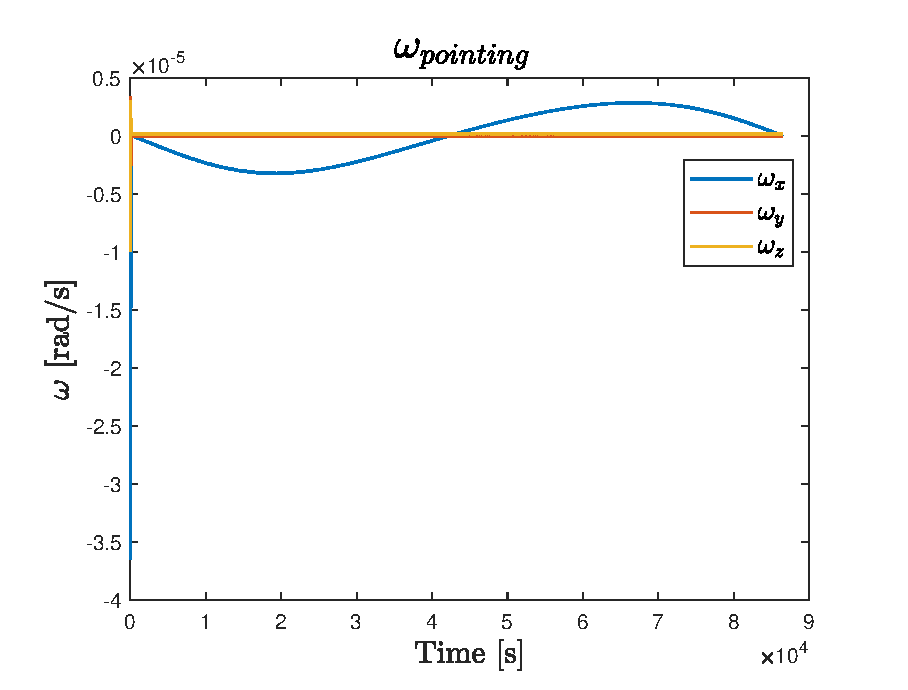
\includegraphics[scale=0.62]{w_pointing.eps}
\caption{ $\omega_{pointing}$  for  1  day}
\end{figure}
\end{minipage}
\begin{minipage}{.5 \textwidth}
\begin{figure} [H]
\centering 
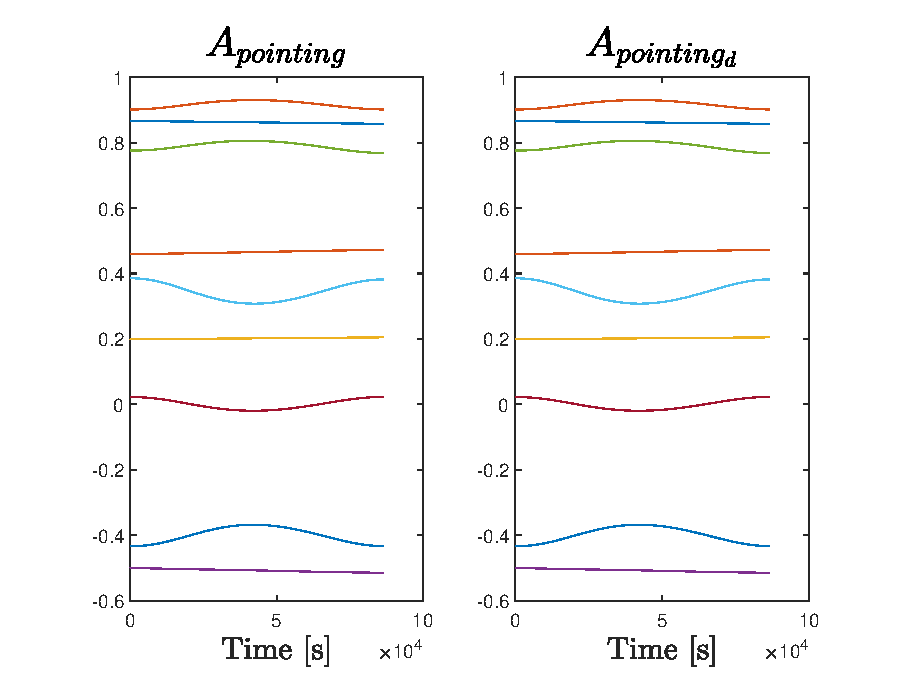
\includegraphics[scale=0.68]{A_poointing.eps}
\caption{ $A_{pointing} \ vs \ A_{desired} $\ for  1 day}
\end{figure}
\end{minipage}\\\\
Firstly the pointing part is simulated  for one day and there are few features to point out:
\begin{enumerate}
   
    \item The spacecraft is almost in a rest configuration because the rate of change of the $ \mathbf{A}$ matrix of the order of 1 day.
   \item In addition both $ \mathbf{A}$ and $ \mathbf{A}_d$ have a period of one day. This can be explained recalling that the orbit is a GEO with 24 H of revolution period . The  position of the Sun changes a little bit due to the relative motion.
\end{enumerate}
\begin{minipage}{.5 \textwidth}
\begin{figure} [H]
\centering 
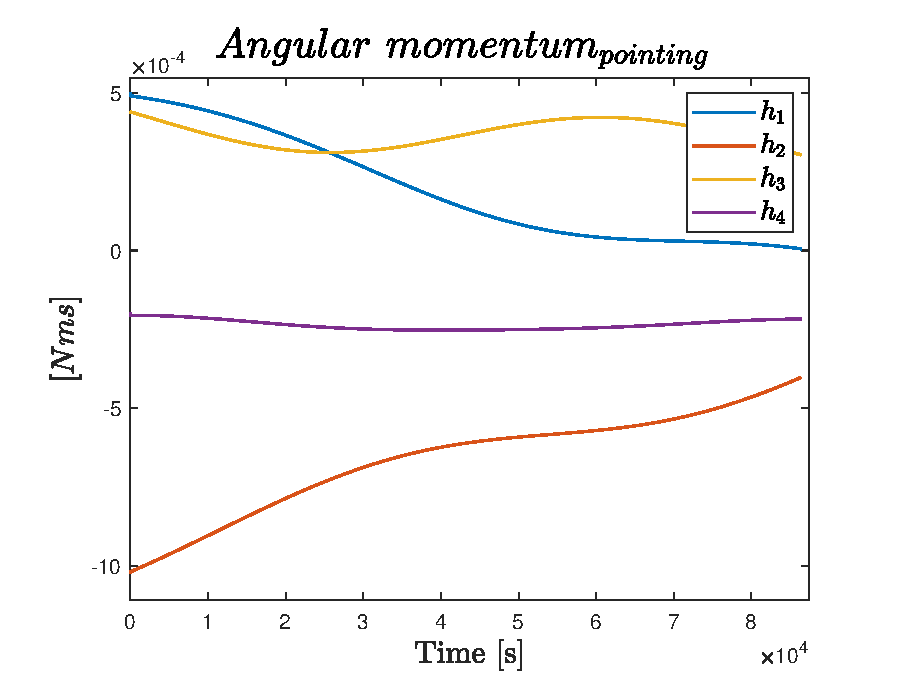
\includegraphics[scale= 0.5]{ang_mom_pointing.eps}
\caption{angular momentum for 1 day}
\end{figure}
\end{minipage}
\begin{minipage}{.5 \textwidth}
Not only does not the slew require the de-saturation of the reaction wheels, but also the pointing. Remember that the maximum angular momentum is set to 10 [mNs]. There are not strong variation in time of the 4 components, because the manoeuvre requires small rotations in 1 day.
\end{minipage}
\begin{minipage}{.5 \textwidth}
\begin{figure} [H]
\centering 
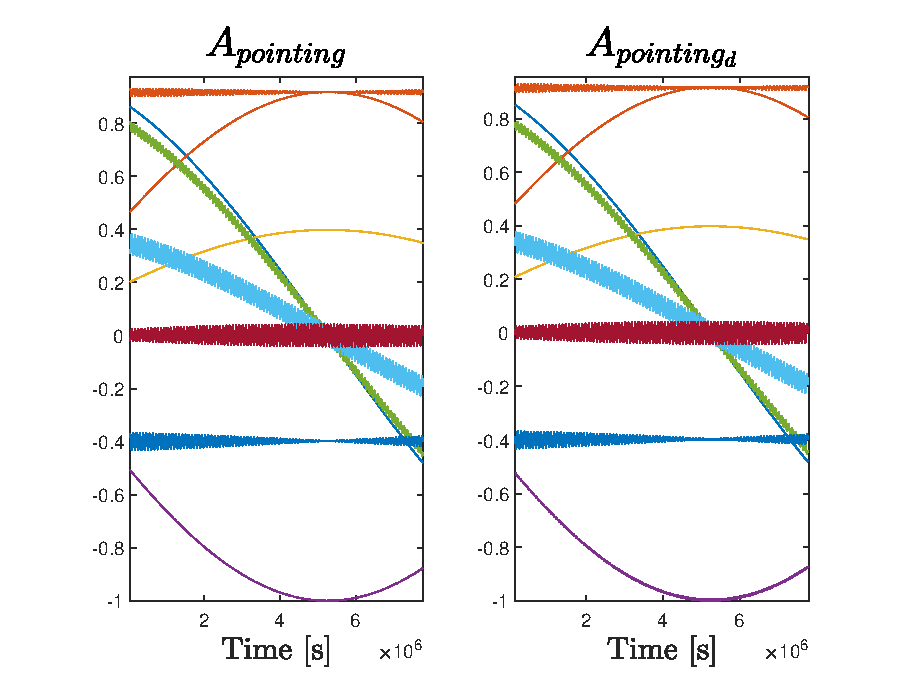
\includegraphics[scale= 0.65]{A_365.eps}
\caption{ $A_{pointing} \ vs \ A_{desired}$ \ for 90 days}
\end{figure}
\end{minipage}
\begin{minipage}{.5 \textwidth}
\begin{figure} [H]
\centering 
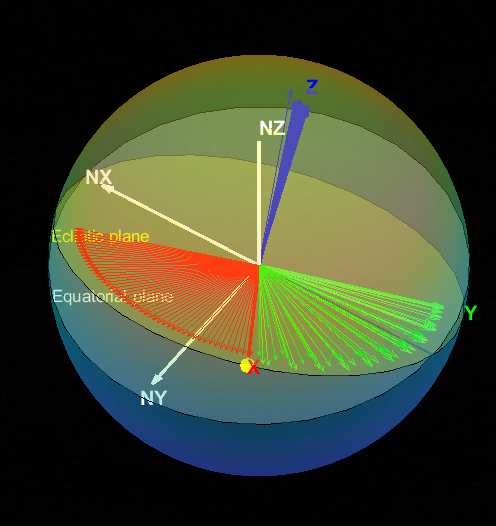
\includegraphics[scale=0.65]{SPHERE_POINTING.PNG}
\caption{ $3_d$ motion}
\label{qwertyuio}
\end{figure}
\end{minipage}\\

Secondly the system  is integrated  for 90 days and it is important underline this aspect: it is possible to notice 2 vibration modes, the former ,at a high frequency,  is brought on by the motion of satellite with respect to the Earth. The latter, at lower frequency, instead is generated by the relative motion of the Sun in the inertial frame.
The \ref{qwertyuio} is the evolution in time of the principal inertial axes in time during tracking.
\section{Conclusions}
Even if a lot of reasonable assumption are made in this project,  the steps may be depicted for the work flow of Cubesat mission. The key point is to merge the requirements of the mission, the equipment available on the market, develop a consistent mathematical a physical model and tune the parameters in a acceptable range trying to get the desired results.Concerning the the output of the Simulink file \ref{results} The control and the actuation is robust against both uncertainties  of the measurements and outer disturbances. Furthermore the system is always able to adapt itself to new requested configurations in a short time. 
\pagebreak
\begin{thebibliography}{}

\bibitem{intro}


Courtesy of \url{https://www.nasa.gov/sites/default/files/atoms/files/nasa_csli_cubesat_101_508.pdf} pp. 9-11 14


 

 \bibitem{6u dimension}
Courtesy of \url{https://static1.squarespace.com/static/5418c831e4b0fa4ecac1bacd/t/5b75dfcd70a6adbee5908fd9/1534451664215/6U_CDS_2018-06-07_rev_1.0.pdf} pp. 25

 \bibitem{gyro}
Courtesy of \url{https://www.sensonor.com/products/inertial-measurement-units/stim300/} 

 \bibitem{structure}
Courtesy of \url{https://www.cubesatshop.com/product/6-unit-cubesat-structure/} 

\bibitem{magnetometer}
Courtesy of \url{https://www.cubesatshop.com/product/nss-magnetometer/} 


\bibitem{magneto_torque}
Courtesy of \url{https://www.cubesatshop.com/product/nctr-m012-magnetorquer-rod/} 

\bibitem{reaction_w_medium}
Courtesy of \url{https://www.cubesatshop.com/product/cubewheel-medium/} 

\bibitem{reaction_w}
Biggs,D.,J.,\textit{Lab 9 slew motions with CMG and RW}, Course of Spacecraft attitude Dynamics And Control, pp 5, 2018

\bibitem{Vacco}
Courtesy of \url{https://www.cubesat-propulsion.com/wp-content/uploads/2015/10/Hybrid-adn-delta-5.pdf} 


\bibitem{perturbations}
Courtesy of \ :\url{https://www.researchgate.net/figure/Orbital-perturbations-as-a-function-of-altitude_fig6_323245224}
\bibitem{perturbationss}
Courtesy of \ : \url{https://www.slideshare.net/zuliana26/satellite-dynamic-and-control}

\bibitem{ecliptic}
Courtesy of \ :\url{https://slideplayer.com/slide/9159756/} 

\bibitem{reference_frame}
Biggs,D.,J.,\textit{Supplementary notes of week 3}, Course of Spacecraft attitude Dynamics And Control, pp 2, 2018

\bibitem{GG}
Courtesy of \ :\url{https://www.researchgate.net/figure/Schematic-of-the-effect-of-the-gravity-gradient-torque-on-the-pitch-angular-velocity-with_fig11_288917865} 

\bibitem{SRP}
Biggs,D.,J.,\textit{Supplementary notes of week 6}, Course of Spacecraft attitude Dynamics And Control, pp 4, 2018 

\bibitem{coefficients}
Biggs,D.,J.,\textit{Supplementary notes of week 7}, Course of Spacecraft attitude Dynamics And Control, pp 3, 2018 

\bibitem{Gyro1}
Biggs,D.,J.,\textit{Supplementary notes of week 8}, Course of Spacecraft attitude Dynamics And Control, pp 1, 2018 

\bibitem{MAgneto1}
Biggs,D.,J.,\textit{Supplementary notes of week 10}, Course of Spacecraft attitude Dynamics And Control, pp 1, 2018 

\bibitem{RW1}
Biggs,D.,J.,\textit{Supplementary notes of week 9}, Course of Spacecraft attitude Dynamics And Control, pp 12, 2018 
\bibitem{riccati}
Courtesy of : \url{http://cdn.intechopen.com/pdfs/39345/intech-optimal_solution_to_matrix_riccati_equation_for_kalman_filter_implementation.pdf}
 \end{thebibliography}{}

 





\end{document}
